\documentclass[runningheads]{llncs}
\usepackage[T1]{fontenc}

% define lightgray
\usepackage[table]{xcolor}

\usepackage{booktabs}
\usepackage[square,sort,comma,numbers]{natbib}
\usepackage[pdfstartview=XYZ,
bookmarks=true,
colorlinks=true,
linkcolor=blue,
urlcolor=blue,
citecolor=blue,
pdftex,
bookmarks=true,
linktocpage=true, % makes the page number as hyperlink in table of content
hyperindex=true
]{hyperref}

\usepackage{orcidlink} % orcidlink
\usepackage{marvosym} %letter symbol
\usepackage{rotating} % Rotating table
\usepackage{subcaption}
\usepackage{graphicx}
\usepackage{multirow}

\usepackage{amsmath}

\newcommand{\myvec}[1]{\mathbf{#1}}

\newcommand{\jd}[1]{\scriptsize {\bf \color{red}[JD: #1]}\normalsize}

\newcommand{\mn}[1]{\scriptsize {\bf \color{blue}[MN: #1]}\normalsize}


\title{Generating synthetic data is complicated: Know your data and know your generator}
\titlerunning{Generating synthetic data is complicated}

\author{Jonathan Latner\inst{1 (\text{\Letter})\orcidlink{0000-0002-1825-0097}} \and
Marcel Neunhoeffer\inst{1 \orcidlink{0000-0002-9137-5785}}  \and
Jörg Drechsler\inst{1 \orcidlink{0009-0009-5790-3394}}}

\authorrunning{Latner et al., \the\year}

\institute{Institute for Employment Research, Nuremberg, Germany
\email{\{jonathan.latner, marcel.neunhoeffer,joerg.drechsler\}@iab.de}}

\begin{document}

\maketitle % typeset the header of the contribution

\begin{abstract} %The abstract should briefly summarize the contents of the paper in 150--250 words.

There is a widely held perception that generating synthetic data are easy.  We argue that generating synthetic data are hard.  Generating synthetic data is a complicated process that requires one to understand both the original dataset and the synthetic data generator (SDG).  In this study, we compare four measures of utility from three SDGs applied to one dataset.  Compared to previous research, the data we use have both higher levels of dimensionality (rows and columns) and contain characteristics found in real data, such messy variables and messy values.  We make two contributions to the literature in this topic area.  First, it is just as important to preprocess or clean the data as it is to tune the SDG in order to create synthetic data with high levels of utility.  Second, we identify a new type of trade-off.  While it is possible to design SDGs that perform well on any one measure of utility, it is not yet possible to design SDGs that perform well on all four measures of utility.  In particular, we highlight the importance of computational efficiency or the duration in time required to generate the synthetic data.  It has long been understood that there is a trade-off between synthetic data with high levels of statistical utility and high levels of privacy protection, but we show that users who want to create synthetic data must also trade-off different types of statistical utility when comparing the advantages and disadvantages of a given SDG.  

\keywords{Data synthesis \and Data utility \and Microdata}
\end{abstract}



% LENGTH OF SUBMISSIONS.

% Using the above format with 11-point font, the paper should be at most 12 pages excluding the bibliography and appendices, and at most 16 pages total. Committee members are not required to read appendices; the paper should be intelligible without them. Submissions not meeting these guidelines risk rejection without consideration of their merits.

\clearpage
\section{Introduction}

\begin{itemize}
    \item \url{Gretel.ai}: The synthetic data platform for developers. Generate artificial datasets with the same characteristics as real data, so you can develop and test AI models without compromising privacy.
    \item \url{Mostly.ai}: Synthetic Data. Better than real. Still struggling with real data? Use existing data for synthetic data generation. Synthetic data is more accessible, more flexible, and simply...smarter.
    \item \url{Statice.ai}: Generating synthetic data comes down to learning the joint probability distribution in an original, real dataset to generate a new dataset with the same distribution.  The more complex the real dataset, the more difficult it is to map dependencies correctly. Deep learning models such as generative adversarial networks (GAN) and variational autoencoders (VAE) are well suited for synthetic data generation.
    \item \url{hazy.com}: Synthetic data does not contain any real data points so can be shared freely. Say goodbye to lengthy governance processes associated with real data.  Specifically, Hazy data is designed to preserve all the patterns, statistical properties and correlations in the source data, so that it can be used as a drop-in replacement for it.
    \item DataSynthesizer: The distinguishing feature of DataSynthesizer is its usability — the data owner does not have to specify any parameters to start generating and sharing data safely and effectively  \cite{ping2017datasynthesizer}.
\end{itemize}


The idea of releasing synthetic data instead of actual data is often understood to have begun in the early 1990s \cite{rubin1993statistical,little1993statistical}.\footnote{We note that several years before Rubin's seminal paper \cite{rubin1993statistical}, an approach was developed for statistical disclosure protection that we might recognize as synthetic data, but they never called it that way \cite{liew1985data}.}  Here, when we refer to data, we are referring to microdata (i.e. one observation per individual unit) as opposed to tabular data (i.e. summary data).  Releasing synthetic data means fitting a model to the original data and then generating new data based on this model so that the released data do not contain information on a real individual unit (person, firm, etc.) that would reveal information that could be used to identify the unit.  The appeal is that the synthetic data mimic the statistical properties of the original data while maintaining the privacy of individual records.

As the quotes above illustrate, there is a general perception that making synthetic data are easy.  Our goal is to explain why making synthetic data are complicated.  There are two reasons.  First, one needs to know the data to be synthesized.  Second, one needs to understand the synthetic data generator (SDG).   Using three SDGs and one dataset, we illustrate the problems that can result when there is a disconnect between knowledge of the data and knowledge of the generator.  Our conclusion: Generating synthetic data is easier than ever. But, to generate good synthetic data, scientists need to have a detailed understanding how and for what purpose the synthetic data are generated.

\section{Study design}\label{sec:study_design}

In this study, we compare four measures of utility from three synthetic data generators (SDGs) applied to one dataset.  In section \ref{sec:know_your_data}, we describe the data.  In section \ref{sec:know_your_generator}, we describe the SDGs.  In this section, we describe the methods.  We assess the utility of the synthetic data using four measures, three of which are propensity mean squared error (pMSE), the ratio of estimates (ROE), and confidence interval overlaps (CIO).  These three utility measures follow Taub et al. \cite{taub2020impact} and Little et al. \cite{little2022comparing}, and are implemented in \textsf{R} from the Synthpop package that compare 5 copies of synthetic data to the original data.  The fourth is the duration in time required to create the synthetic dataset \cite{jordon2022synthetic}.  The combination of measures illustrates the trade-off users must make between the advantages and disadvantages each of the SDGs.

The propensity score \cite{woo2009global,snoke2018general} (pMSE) is a parametric utility measure that estimates how well one can discriminate between the original and synthetic data based on a classifier.  This is sometimes called a `broad'\cite{snoke2018general} or `general'\cite{drechsler2009disclosure} measure of utility or `statistical fidelity' \cite{jordon2022synthetic}.  The main steps are to append or stack the original and the synthetic data, add an indicator (1/0) to distinguish between the two, use logistic regression to estimate the propensity of each record in the combined dataset being `assigned' to the original data, and compare the distributions of the estimated propensity score in the two datasets.  In summary:

%%%%%%%%%%%%%%%%%%%%%%%%%%%%%%%%%%%%%%%%%%
\begin{equation}
pMSE = \frac{1}{N}\sum_{i=1}^{N}[\hat{p}_i - c]^2
\end{equation}
%%%%%%%%%%%%%%%%%%%%%%%%%%%%%%%%%%%%%%%%%%
where $N$ is the number of records in the combined dataset, $\hat{p}_i$ is the estimated propensity score for record $i$, and $c$ is the proportion of data in the merged dataset that is synthetic (0.5). pMSE can be estimated on the complete dataset or subsets of the variables, e.g., all one-way, two-way or three-way combinations. The smaller the pMSE, the higher the analytical validity of the synthetic data.

Ratio of estimates (ROE) is a non-parametric utility measure that compares estimates (frequency or proportion) of values within a variable between the original and synthetic data.\footnote{\url{https://github.com/clairelittle/psd2022-comparing-utility-risk/blob/main/code/ROC_Ratio_of_Counts_Estimates.R}}  The three main steps are (1) create a frequency table (one- or two-way) for the same variable(s) in the synthetic and original data.  (2) Within each table, compare the two estimates for each value by dividing the smaller of these two estimates by the larger one.  (3) Average the resulting within table proportions.  In summary:

%%%%%%%%%%%%%%%%%%%%%%%%%%%%%%%%%%%%%%%%%%
\begin{equation}
    ROE = \frac{1}{N} \sum^{N}_{i=1} \left( \frac{\text{min}(y_{orig}^i,y_{synth}^i)}{\text{max}(y_{orig}^i,y_{synth}^i)} \right)
\end{equation}
%%%%%%%%%%%%%%%%%%%%%%%%%%%%%%%%%%%%%%%%%%
where $N$ is the number of values within a table, $y^i_{orig}$ is the estimate from the original data and $y^i_{synth}$ is the corresponding estimate from the synthetic data.  The higher the ROE, the higher the analytical validity of the synthetic data.  

The confidence interval overlap (CIO) is a parametric utility measure that compares 95\% confidence intervals between the same regression model applied to synthetic and original data \cite{karr2006framework}.  This is sometimes called a `specific'\cite{snoke2018general} or `narrow'\cite{drechsler2009disclosure} measure of utility.  The main steps are to average the difference between the upper and lower bound estimates of the confidence interval for each independent variable in the model.\footnote{\url{https://github.com/clairelittle/psd2022-comparing-utility-risk/blob/main/code/CIO_Confidence_Interval_Overlap.R}} In summary:

%%%%%%%%%%%%%%%%%%%%%%%%%%%%%%%%%%%%%%%%%%
\begin{equation}
    CIO = \frac{1}{N} \sum^{N}_{i=1} \frac{1}{2}\left(\frac{\text{min}(u_o,u_s) - \text{max}(l_o,l_s)}{u_o-l_o} + \frac{\text{min}(u_o,u_s) - \text{max}(l_o,l_s)}{u_s-l_s}\right)
\end{equation}
%%%%%%%%%%%%%%%%%%%%%%%%%%%%%%%%%%%%%%%%%%
where $N$ is the number of independent variables, and $u_o,l_o$ and $u_s,l_s$ are the respective upper and lower bounds of the confidence intervals for the original and synthetic data.   The higher the CIO, the higher the analytical validity of the synthetic data.  

Our fourth utility measure is the duration in time (in seconds) required to create one single synthetic dataset from a given SDG.\footnote{In terms of computing power, SDGs were run on a 2022 Macbook Air with 16GB of RAM and an M2 Chip with 8‑Core CPU, 8‑Core GPU, and a 16‑Core Neural Engine.  All SDGs were run one at a time in order to minimize computational power problems from parallelization.}  We refer to duration as computational efficiency, but it is sometimes referred to as `efficiency'\cite{jordon2022synthetic} or `output scalability'\cite{zhang2017privbayes}.  The basic idea is that the algorithms used by SDGs can suffer from the curse of dimensionality.\footnote{``a million row table with ten attributes, each of which has 20 possible values, results in a domain size (and hence an output size) of $m = 20^{10} \approx 10$TB, which is $\dots$ slow to use compared to the input that can be measured in megabytes.'' \cite{zhang2017privbayes}}  Therefore, SDGs that are appropriate for some datasets are not appropriate for others.  

It has long been understood that there is a trade-off between synthetic data with high levels of statistical utility and high levels of privacy protection.  It is less understood is that users who want to create synthetic data must also trade-off different types of statistical utility when comparing the advantages and disadvantages of a given SDG.  While it is possible to design SDGs that perform well on any one measure of utility, it is not yet possible to design SDGs that perform well on all measures of utility \cite{drechsler2022challenges,jordon2022synthetic}.  


\section{Know your data}\label{sec:know_your_data}

The data we use are called, Social Diagnosis 2011 - Objective and Subjective Quality of Life in Poland (SD2011).  The data are included as part of the Synthpop package.\footnote{We note that the data are publicly available here: \url{http://www.diagnoza.com/index-en.html}.  However, we are as yet unable to replicate data made available from the Synthpop package from the raw data.}  As shown in table \ref{table:sd2011_data_structure}, there are 35 variables and 5.000 observations, 21 variables are categorical (or factor), and 14 variables are numeric.  There are two main reasons why SD2011 data are helpful to illustrate the potential problems that may exist in the disconnect between knowledge of the data and knowledge of the synthetic data generator (SDG).  

One is data dimensionality. Compared to previous evaluations \cite{dankar2021fake,little2022comparing}, SD2011 contain the highest dimensional dataset with respect to rows and columns.  While previous research used data with more columns ($> 40$), the data contained far fewer rows ($< 1.000$) or if data contained more rows (32.000), then they contained fewer columns (25).  Further, the data contain a factor variable (\texttt{eduspec}) and a continuous variable (\texttt{wkabdur}) with a large number of unique values.  Data dimensionality affects the duration in time required to generate the synthetic data, which we refer to in this paper as computational efficiency.  While the number of rows and columns may not seem like high-dimensional data, we will show that a SDG can struggle to create synthetic data with these dimensions.

The second reason is that SD2011 contain many properties of real data, including missing, `messy' or extreme values, and generated variables.  These properties are both independent and related.  Previous evaluations use clean data from Census \cite{little2022comparing} or machine learning libraries (Kaggle, UCI, OpenML) \cite{dankar2021fake}.  Without denying the value of clean data for evaluation purposes, real data illustrate challenges of using SDGs that would not otherwise be understood.  

Missing values present two main challenges.  One is that some SDGs cannot be used on data with missing values.  Therefore, the ability to synthesize missing values is a stage of development that SDGs must pass through before they can be applied to real data.\footnote{Early versions CTGAN could not be used on data with missing values.\footnote{\url{https://github.com/sdv-dev/CTGAN/issues/39}}}  Another is that it is not always clear what values are missing or what missing values mean.  For example, factor variables contain missing values and numeric variables contain negative values that we assume are missing.  However, \texttt{income} is a numeric variable that contains both missing and negative values.   Further, there is the issue of `informed missings.'  For example, the variable for total time spent working abroad (\texttt{wkabdur}) is missing if an individual did not work abroad (\texttt{wkab} = Y/N).  The correct coding of missing values when creating synthetic data requires knowledge of the data that is not always available and may not be easy or possible to detect or follow simple rules.

Generated variables are variables created from the original values.  In SD2011, there are two generated variables.  The variable \texttt{agegr} is generated from \texttt{age} and the variable \texttt{bmi} is generated from \texttt{height}(cm) and \texttt{weight}(kg).  Given that synthesizing any one variable is a challenge, the challenge increases for each additional variable being synthesized, by definition.  It is not necessary to synthesize generated variables, but generated variables require knowledge of the data and cannot be detected by the SDG.  

Messy variables also exist that contain values that are outliers or errors.  For example, in the case of \texttt{bmi}, there is an outlier value of 450, which is the result of height of 149 and missing weight.  If we calculate weight from bmi and height, then weight equals 999 or one metric ton.  The existence of outlier values can affect the ability of SDGs to create synthetic data with high levels of utility as well as privacy.  An example of an error are the variables for \texttt{smoke} and \texttt{nociga}, where two individuals indicate they do not smoke also indicate they smoke 20 or 22 cigarettes per day, respectively.  Given the importance of outliers on results, it is important to distinguish outliers from errors when synthesizing data

Finally, while it is easy to label variables as categorical or continuous, some continuous variables can look like categorical variables and visa versa.  For example, the variable for \texttt{nofriend} is a continuous variable for the number of friends a survey respondent has.  As we will show later, values below 10 are normally distributed, but then cluster at 10, 20, and so on.  Another example is the variable for \texttt{wkabdur} or `total time spent working abroad', which is a numeric variable that Synthpop treats as a factor variable.  While it is understood that certain SDGs are more or less appropriate for certain variable types, variation exists within variable types that can also affect utility of a given SDG. 

In summary, SD2011 is a useful dataset to compare and contrast the advantages and disadvantages of SDGs in a real setting.  We use three versions of the original data to create synthetic data and compare utility.  SD2011(a) is the raw data.  SD2011(b) codes all negative values in numeric variables as missing and all empty values in character variables as missing.  SD2011(c) drops the two generated variables: \texttt{agegr} and \texttt{bmi}.

\section{Know your generator}\label{sec:know_your_generator}

In this section, we tune three synthetic data generators (SDGs) to find optimal utility within a given SDG on our SD2011 data.  The three SDGs we use are commonly compared and contrasted in the literature \cite{dankar2021fake,little2022comparing}.  While we describe the process of tuning the hyperparameters in the main body of the text, most of the supporting figures are in the respective subsections of online appendix.  

\subsection{DataSynthesizer}\label{subsec:know_your_generator_datasynthesizer}

DataSynthesizer (Version 0.1.11) was used \cite{ping2017datasynthesizer}, which implements the PrivBayes algorithm \cite{zhang2017privbayes}.  DataSynthesizer is designed to address the challenges associated with creating synthetic data outputs from high-dimensional real data inputs.  To achieve this goal, the package implements a Bayesian network model.  Like most Bayesian network structures \cite{chen2017learning}, DataSynthesizer algorithms assume that all variables are discrete and continuous variables are encoded or discretized (the default value is 20 bins).  Afterward, values for continuous variables are re-encoded within a given bin.  Therefore, the ability to maintain output scalability with dimensionality is partially derived by sacrificing some amount of utility in continuous variables.   

There are a number of hyperparameters that might be tuned for DataSynthesizer, but we focus on two, with all other values set to default.  One hyperparemeter is differential privacy ($\epsilon$-DP). This is a number that quantifies the amount of noise that is introduced into the original data to create synthetic data.  In Datasynthesizer, the default is 0.1 and 0 turns off DP.  We turn off DP in order to compare to the other synthesizers that do not have a similar hyperparameter.  

A second hyperparameter are the number of attributes any one variable can have, i.e. parents ($k$).  In a Bayesian Network, there are three possible relationships between X and Y.  Direct dependence where each variable can only have direct attributes (1 parent), weak conditional independence where each variable can have both direct and indirect attributes (2+ parents), and strong conditional independence where all variables are independent (0 parents).  

As a first step, we tune DataSynthesizer on SD2011(a) based on the number of parents in the Bayesian network with pMSE as a utility measure (lower values are better), as shown in figure \ref{fig:tuning_ds_dataset} in the online appendix \ref{appendix:datasynethsizer}.  For 0 and 1 parents, pMSE = 0.25; pMSE = 0.2 with 2 parents; and pMSE = 0.21 for 3 parents.  Therefore, 2 parents represents the optimal level of utility.

As a second step, we estimate pMSE for all two-way combinations of variables in SD2011(a), as shown in figure \ref{subfig:ds_fidelity_two_way_subfig-a}.  While most values are close to 0, it is clear that synthetic values do not match well with original values for the variable, \texttt{wkabdur} (work abroad duration).  In the original data, 0.975\% of all values are -8, as shown in figure \ref{subfig:ds_variable_wkabdur}.  The problem is that DataSynthesizer not only creates synthetic values of -8, but also values between -8 and 0 that do not exist in the original data.  Therefore, we code all negative values in numeric variables as missing and all empty values in character variables as missing to create SD2011(b).

Next, we re-estimate pMSE for all two-way combinations of variables in SD2011(b), as shown in figure \ref{subfig:ds_fidelity_two_way_subfig-b}.  While most values are close to 0, it is clear that synthetic values do not match well with original values for the variable, \texttt{bmi} (body mass index).  In the original data, the variable \texttt{bmi} contains a single value of 450, as shown in figure \ref{subfig:ds_variable_bmi}.  This is an extreme value that is nearly 6 times larger than the next closest value of 76.  Similar to the variable, \texttt{wkabdur}, the problem is that DataSynthesizer not only creates synthetic values of 450, but also values between 76 and 450 that do not exist in the original data.  Fortunately, \texttt{bmi} is one of two generated variables (the other is \texttt{agegr}) that are created based on other variables in the data.  Given that these are unnecessary to synthesize, we drop both generated variables (\texttt{bmi} and \texttt{agegr}) to create SD2011(c).

Finally, we re-estimate pMSE for all two-way combinations of variables in SD2011(c), as shown in figure \ref{subfig:ds_fidelity_two_way_subfig-c}.  While most values are close to 0, it is clear that synthetic values do not match well with original values for the variable, \texttt{nofriend} (number of friends).  In section \ref{sec:results}, we will explain why DataSynthesizer does not create good synthetic values for the variable, \texttt{nofriend}.  To continue to improve the utility of DataSynthesizer, one solution would be to drop the variable or make further changes to clean or preprocess it.  However, this would require comparatively more research choice relative to the other steps we took.  Therefore, we make no further changes and SD2011(c) is our main data.

In summary, this exercise illustrates two key points.  First, one must know the data.  Missing, negative, or extreme values as well as the presence of generated variables affect the similarity or difference between the synthetic and original data.  If we compare pMSE across the three versions of SD2011, then  pMSE = 0.21 for SD2011(a), pMSE = 0.13 for SD2011(b), and pMSE = 0.07 for SD2011(c), as shown in figure \ref{fig:tuning_ds_optimize_dataset_compare}.  Second, one must know the generator.  The reason why some variables in the synthetic data did not match well with the original data is because the Bayesian network implemented by DataSynthesizer discretizes continuous variables into bins and then re-encodes values within a given bin, which affects the utility of the synthetic data.  Therefore, preprocessing the data is at least as important as tuning the synthesizer.

\subsection{CTGAN} 

CTGAN (Version 1.9.0) was used \cite{ctgan}.  CTGAN is part of the Synthetic Data Vault package \cite{patki2016synthetic}.  In their original application, GANs were designed to create synthetic images  \cite{goodfellow2014generative}, but the approach was adapted to create synthetic microdata \cite{park2018data}.  GANs simultaneously train two neural networks: a generator and a discriminator. The goal of the generator is to create synthetic data that becomes increasingly indistinguishable from original data.  The goal of the discriminator is to get better at distinguishing between original and synthetic data.  This adversarial process goes back and forth until the discriminator cannot distinguish between the original data and the generated data.  One advantage is that GANs are designed to work well continuous variables, unlike DataSynthesizer.  One disadvantage is that cells in micro data are not informative of neighbors in the same way that pixel cells in a photograph. As a result, GANs can struggle modeling relationships between cells and columns \cite{drechsler202330}.

CTGAN contains a number of hyperparameters that one can use to tune the model. Following the package authors, we distinguish between two types of hyperparameters: `primary' and `advanced'.  The primary one is the number of steps contained in the model, which is a function of the number of observations in the original data and two hyperparameters: Epochs and Batch size.  In the default, batch size is 500 and epochs is 300.  With 5.000 observations in the original data (SD2011), this means that it takes 10 steps within each Epoch to examine the entire data frame (5000/500=10) and the total number of steps is 3.000 (10*300).  Too few epochs may result in underfitting and too many epochs may result in overfitting.

Advanced hyperparameters include the dimensionality and embedding dimension, but others exist (i.e learning rate, and weight decay, etc.).  The dimensionality is the number of layers in the generator/discriminator networks.  A fully connected layer will be created for each one of the values provided (default is [256,256]).  Technically, one can vary the values for both the dimensionality of the discriminator and generator, but we set the same value for both.  The embedding dimension influences how much the information in the original dataset is compressed.  For example, an embedding dimension of 1 is equivalent to storing 33 columns of data in SD2011(c) in a single number (default is 128).

As shown in figure \ref{fig:ctgan_fidelity_optimize} in online Appendix \ref{appendix:CTGAN}, we tune the hyperparameters in three main ways.  First, we maintain a constant number of steps (3.000), but allow the batch size to vary (figure \ref{subfig:ctgan_fidelity_optimize_batch_size}).  Second, we maintain a constant batch size (500), but allow the steps to vary (figure \ref{subfig:ctgan_fidelity_optimize_epochs}).  Third and finally, we vary the dimensionality of the generator/discriminator networks and the embedding dimension (figure \ref{subfig:ctgan_fidelity_optimize_dimensions}).  In our data (SD2011), tuning these hyperparameters makes little difference (levels pMSE $\approx$ 0.16).  Given that, we maintain default values for all hyperparameters with the exception of epochs, which we increase to 600.

In summary, this exercise illustrates two key points.  First, tuning CTGAN made little difference in the utility of the synthetic data.  We are aware of other, similar research (as yet unpublished) where tuning CTGAN did make a difference.  One possible explanation is that our data contain a relatively small number of observations (5.000).  Second, we note that pMSE is about twice as high as our optimized SDG using DataSynthesizer.  The interpretation is that CTGAN is not a very good synthesizer.  However, as described earlier, CTGAN is not the only GAN one can use to create synthetic microdata.  Evidence (as yet unpublished) suggests it is possible to create a better GAN.

\subsection{Synthpop} 

Synthpop (Version 1.8.0) \cite{nowok2016synthpop} was used. Synthpop is an \textsf{R} package that implements parametric and CART models (classification and regression trees) to generate synthetic data.  CART models are the default.  Synthpop follows the two-stage process described by Rubin \citep{rubin1993statistical}, where the variables in the dataset are synthesized one at a time, sequentially.  Evaluations often find that Synthpop/CART models appear to create synthetic data that are statistically more similar to original data than other SDGs  \cite{little2022comparing,dankar2021fake,drechsler2011empirical}.  However, Synthpop, like all SDGs contains advantages and disadvantages.  The advantage is one can easily create synthetic data with high levels of utility and little tuning, but the disadvantage is that CART and tree-based models in general struggle computationally with variables that contain many categories  \cite{little2022comparing}.  Given that tuning hyperparameters cannot help improve computational efficiency and has little effect on statistical utility, we use default values for all hyperparameters in Synthpop.


%First, a model for predicting a given outcome variable ($y$) given a set of background variables ($x$) is trained on the actual data.  Second, values of the original outcome variable are replaced by random draws from the model of the outcome variable ($y^*$).  This process is then repeated so that all actual values are replaced by imputed values for every variable.  The result is a synthetic dataset that contains no values in the actual data, but is statistically similar to the original data, not only with respect to mean and variation within a given variable, but also correlations between variables.  



\section{Results from comparing SDGs}\label{sec:results}

In this section, we compare our three synthetic data generators (SDGs) on our four measures of utility using one dataset.  We begin by comparing pMSE (lower values are better) across our optimized SDGs, as shown in figure \ref{subfig:graph_fidelity_compare_dataset}.  pMSE = 0.15 for CTGAN, 0.07 for DataSynthesizer, and 0.02 for Synthpop.  More detail is visible in figure  \ref{subfig:graph_fidelity_compare_twoway} that compares two-way pMSE for all variables in the data for each SDG.  In CTGAN, values are close to 0.075 for most variables.  In DataSynthesizer, values are close to zero for most variables except the variable, \texttt{nofriend} (number of friends).  In Synthpop, values are close to zero for most variables.  The interpretation is that synthetic data from Synthpop is much closer to the original data (SD2011c) than synthetic data created by CTGAN or DataSynthesizer.

Next, we examine one-way frequency statistics and the ratio of estimates (ROE -  higher values are better) for select variables to better understand how different SDGs estimate synthetic values, as shown in figure \ref{fig:graph_frequency_compare}.  We select four variables to highlight the issues of synthesizing different types of variables. 

We begin with  the normally distributed variable, \texttt{bmi} (Body mass index), as shown in figure \ref{subfig:graph_frequency_compare_bmi}.  While \texttt{bmi} was dropped from the original data prior to generating synthetic data for reasons specified in section \ref{subsec:know_your_generator_datasynthesizer}, it was added back after the synthetic data was created by combining synthesized values for height and weight.  If we examine ROE values for the variable  \texttt{bmi} from table \ref{table:table_compare_roe}, then ROE = 0.4 for Synthpop, ROE = 0.28 for CTGAN, and 0.17 for DataSynthesize, then ROE = 0.21 for both CTGAN and DataSynthesizer, and ROE = 0.24 for Synthpop.  The interpretation is that all three SDGs provide similar levels of utility when synthesizing a continuous variable with a normal distribution, even if Synthpop is slightly better.  

Next, we examine the categorical variable, \texttt{edu} (Education), as shown in figure \ref{subfig:graph_frequency_compare_edu}.  Visually, it appears that all three SDGs provide comparable synthetic values to the original data.  If we examine ROE values for the variable \texttt{edu} from table \ref{table:table_compare_roe}, ROE = 0.88 for CTGAN, ROE = .99 for DataSynthesizer, and ROE = 0.94 for Synthpop.  We note that all values are higher than the continuous variable (\texttt{bmi}).  The interpretation is that all three SDGs provide similar levels of utility when synthesizing a categorical variable, even if DataSynthesizer is slightly better.  

We get a different picture of SDG quality when we look at a continuous variable with a non-uniform distribution,  \texttt{nofriend} (number of friends), as shown in \ref{subfig:graph_frequency_compare_nofriend}.  In the original data, the variable \texttt{nofriend} appears to be normally distributed below 10, but then clusters at values of 10, 15, 20 and groups of 10 up to the maximum 99.  In values below 30, Synthpop and CTGAN perform similarly well, but DataSynthesizer does not capture clustering or discontinuity in the variable.  Instead, DataSynthesizer replaces real values with values that are normally distributed.  In values above 30, Synthpop still performs well, but CTGAN and DataSynthesizer do not.  If we examine ROE values for the variable  \texttt{nofriend} from table \ref{table:table_compare_roe}, then ROE = 0.4 for Synthpop, ROE = 0.28 for CTGAN, and 0.17 for DataSynthesizer.  The interpretation is that Synthpop creates synthetic values for the variable \texttt{nofriend} that are closer to the original values than either CTGAN or DataSynthesizer.

The last variable we examine is \texttt{wkabdur} (Work abroad duration), which allows us to examine the challenge of synthesizing variables that contain `informed missings.'  Values refer to the number of weeks a survey respondent worked abroad between 2007 and 2011, as shown in figure \ref{subfig:graph_frequency_compare_wkabdur}.  Nearly 98\% of all values are missing, indicating that a respondent did not work abroad.  In the original data the mean is 14 and the median is 10, but both Synthpop and CTGAN overestimate the median as 14.  If we examine ROE values for the variable  \texttt{wkabdur} from table \ref{table:table_compare_roe}, then ROE = 0.059 for CTGAN, ROE = 0.287 for DataSynthesizer, and ROE = 0.38 for Synthpop.  Synthpop is captures the distribution of nonmissing values better than DataSynthesizer or CTGAN.

Figure \ref{fig:utility_compare_cio} displays parameter estimates and confidence interval overlap (CIO) for two regression models, an OLS model where the dependent variable is continuous (\texttt{LN(Income)}) and a GLM model where the dependent variable is dichotomous (\texttt{smoke}).  In both models, the independent variables are \texttt{gender}, \texttt{age}, \texttt{education}, and \texttt{bmi}.  In both models, Synthpop has the highest percent of CIO while CTGAN and DataSynthesizer have similarly low levels.  

However, when we examine the parameter estimates from the GLM model, Synthpop, like CTGAN and DataSynthesizer, over estimates the effect of education level on smoking for two values (less than secondary and secondary) as positive and significant.  In the original data, they are positive and insignificant.  The conclusion from synthetic data would be that levels of education affect smoking, but the conclusion from  the original data is that smoking is only related to one level of education (vocational or grammar).  Therefore, while synthetic data from Synthpop better capture parametric relationships in the original data compared to other SDGs, they are not a substitute for real data.

Finally, we compare the duration in time required to create synthetic data from the SDGs, i.e. computational efficiency, as shown in table \ref{table:table_sd2011_duration}.  The first row displays results from the raw data.  CTGAN requires 331 seconds (5 minutes and 30 seconds) and DataSynthesizer requires 245 seconds (4 minutes).  By contrast, duration times from Synthpop are much longer.  If we load SD2011 into \textsf{R} as a .csv file as we do with DataSynthesizer and CTGAN, then Synthpop requires 2,132 seconds (35 minutes and 30 seconds), but we if load SD2011 into \textsf{R} from the Synthpop package, then Synthpop requires 5,474 seconds (91 minutes).

The difference in duration within Synthpop and between Synthpop and the other SDGs is explained by two variables: \texttt{eduspec} and \texttt{wkabdur}.  Both variables have a large number of unique values (28 and 33, respectively).  For some reason when SD2011 is loaded into \textsf{R} from the Synthpop package, then \texttt{wkabdur} is treated as a character variable, not a numeric variable, as it actually is.  However, if SD2011 is loaded into \textsf{R} from a .csv file, then \texttt{wkabdur} is correctly treated as a numeric variable.  The second problem is that Synthpop struggles computationally with variables that contain many categories.  A suggestion by the package authors is to place this variables at the end prior to synthesizing the data \cite{raab2017guidelines}.  When we treat \texttt{wkabdur} as a numeric variable and place \texttt{eduspec} at the end, then Synthpop requires less than 15 seconds, regardless of how SD2011 is loaded.  Therefore, Synthpop is more computationally efficient with SD2011 than either CTGAN or DataSynthesizer with proper preprocessing.

However, the issue reveals a more general problem: unlike CTGAN and DataSynthesizer, Synthpop is sensitive to the number (and order) of categorical variables with large values.  To illustrate this, we added one, two, or three categorical variables with 20, 25, or 30 unique random categorical values to SD2011.  While duration times for CTGAN and DataSynthesizer are almost insensitive to the number of categorical variables or unique values, duration times for Synthpop increase with additional variable and number of unique values.  Therefore, Synthpop is less computationally efficient as the data dimensions increase. 

\section{Conclusion}\label{sec:conclusion}

In contrast to the simplicity of the original idea, and despite decades of progress, the creation of synthetic data include steps that are neither common knowledge nor described in one place.  The conclusion is that making synthetic data is complicated and requires knowledge that may not always exist in one place.  

One must know the data.  Most research examining synthetic data generators (SDGs) uses clean data from Census or Machine Learning libraries.  Unlike clean data, real data contain variables with messy values, which can affect the utility of SDGs.  Despite advertisments to the contrary, it is not possible to simply input real data into a SDG or and high expect high quality synthetic data output.  Our results show that utility of synthetic data is a result of both preprocessing the data and tuning a SDG.  

One must know the generator.  There is no one size fits all solution and choosing the right SDG is the result of different trade-offs.  For example, our results clearly show that Synthpop produces synthetic data with the highest level of utility among all three SDGs, but the CART method that Synthpop uses as the default struggles with computational efficiency with datasets that contain variables with many categories.  It is difficult to imagine applying Synthpop to so-called `big data' with hundreds of variables and millions of observations.  By contrast, even though DataSynthesizer generates synthetic data with lower levels of utility, it is designed to perform well on high dimensional data.  One may need to trade-off computational efficiency with statistical utility.

CTGAN is not good, but that does not mean GANs are bad.  Our results suggest that CTGAN provides the lowest levels of utility of any of the three SDGs we examined.  However, CTGAN is not the only GAN in Synthetic Data Vault and multiple other GANs exist.  We note a disconnect in the literature on synthetic data between computer scientists that often rely on GANs without comparing them to CART and statisticians that compare GANs to CART and find that CART models are superior \cite{drechsler202330}.  We are aware of GANs that produce synthetic data with similar utility as Synthpop (as yet unpublished).  It is possible to create a GAN that provides higher levels of utility.  More generally, one must distinguish between the package and the method.  

Synthetic data is not a substitute for original data \cite{jordon2022synthetic}.  Our results suggest that Synthpop produces synthetic data with the highest level of utility among the three SDGs, but estimated coefficients from a GLM model applied to synthetic data produce results that are not consistent with the original data.  Therefore, prior to making synthetic data, one must decide the purpose.



%\subsubsection*{Acknowledgments}
%Use unnumbered third level headings for the acknowledgments. All acknowledgments, including those to funding agencies, go at the end of the paper. Only add this information once your submission is accepted and deanonymized. 

%%%%%%%%%%%%%%%%%%%%%%%%%%%%%%%%
% Tables
%%%%%%%%%%%%%%%%%%%%%%%%%%%%%%%%
\clearpage
\section{Tables}

\vskip -5mm
\begin{table}[!htb]
\minipage{\textwidth}
% \begin{table}
    \caption{Social Diagnosis 2011 (SD2011)}
    \centering
    \rowcolors{1}{white}{lightgray}
    \resizebox{\textwidth}{!}{% latex table generated in R 4.4.0 by xtable 1.8-4 package
% Thu Sep 26 09:11:53 2024
\begin{tabular}{rlllllllll}
  \toprule
Number & Variable & Description & Type & Observations & Unique.Values & Missings & Negative.values & Generated & Messy \\ 
  \midrule
  1 & sex & Sex & factor & 5000 & 2 & 0 & 0 &  &  \\ 
    2 & age & Age of person, 2011 & numeric & 5000 & 79 & 0 & 0 &  &  \\ 
    3 & agegr & Age group, 2011 & factor & 5000 & 7 & 4 & 0 & Yes & Yes \\ 
    4 & placesize & Category of the place of residence & factor & 5000 & 6 & 0 & 0 &  &  \\ 
    5 & region & Region (voivodeship) & factor & 5000 & 16 & 0 & 0 &  &  \\ 
    6 & edu & Highest educational qualification, 2011 & factor & 5000 & 5 & 7 & 0 &  &  \\ 
    7 & eduspec & Discipline of completed qualification & factor & 5000 & 28 & 20 & 0 &  &  \\ 
    8 & socprof & Socio-economic status, 2011 & factor & 5000 & 10 & 33 & 0 &  &  \\ 
    9 & unempdur & Total duration of unemployment in the last 2 years (in months) & numeric & 5000 & 30 & 0 & 1556 &  &  \\ 
   10 & income & Personal monthly net income & numeric & 5000 & 407 & 683 & 603 &  & Yes \\ 
   11 & marital & Marital status & factor & 5000 & 7 & 9 & 0 &  &  \\ 
   12 & mmarr & Month of marriage & numeric & 5000 & 13 & 1350 & 0 &  &  \\ 
   13 & ymarr & Year of marriage & numeric & 5000 & 75 & 1320 & 0 &  &  \\ 
   14 & msepdiv & Month of separation/divorce & numeric & 5000 & 13 & 4300 & 0 &  &  \\ 
   15 & ysepdiv & Year of separation/divorce & numeric & 5000 & 51 & 4275 & 0 &  &  \\ 
   16 & ls & Perception of life as a whole & factor & 5000 & 8 & 8 & 0 &  &  \\ 
   17 & depress & Depression symptoms indicator & numeric & 5000 & 23 & 89 & 0 &  &  \\ 
   18 & trust & View on interpersonal trust & factor & 5000 & 4 & 37 & 0 &  &  \\ 
   19 & trustfam & Trust in own family members & factor & 5000 & 4 & 11 & 0 &  &  \\ 
   20 & trustneigh & Trust in neighbours & factor & 5000 & 4 & 11 & 0 &  &  \\ 
   21 & sport & Active engagement in some form of sport or exercise & factor & 5000 & 3 & 41 & 0 &  &  \\ 
   22 & nofriend & Number of friends & numeric & 5000 & 44 & 0 & 41 &  & Yes \\ 
   23 & smoke & Smoking cigarettes & factor & 5000 & 3 & 10 & 0 &  &  \\ 
   24 & nociga & Number of cigarettes smoked per day & numeric & 5000 & 30 & 0 & 3737 &  & Yes \\ 
   25 & alcabuse & Drinking too much alcohol & factor & 5000 & 3 & 7 & 0 &  &  \\ 
   26 & alcsol & Starting to use alcohol to cope with troubles & factor & 5000 & 3 & 82 & 0 &  &  \\ 
   27 & workab & Working abroad in 2007-2011 (in months) & factor & 5000 & 3 & 438 & 0 &  &  \\ 
   28 & wkabdur & Total time spent on working abroad & numeric & 5000 & 33 & 0 & 4875 &  & Yes \\ 
   29 & wkabint & Plans to go abroad to work in the next two years & factor & 5000 & 4 & 36 & 0 &  &  \\ 
   30 & wkabintdur & Intended duration of working abroad & factor & 5000 & 6 & 4697 & 0 &  &  \\ 
   31 & emcc & Intended destination country & factor & 5000 & 18 & 4714 & 0 &  &  \\ 
   32 & englang & Knowledge of English language & factor & 5000 & 4 & 15 & 0 &  &  \\ 
   33 & height & Height of person & numeric & 5000 & 65 & 35 & 0 &  &  \\ 
   34 & weight & Weight of person & numeric & 5000 & 91 & 53 & 0 &  &  \\ 
   35 & bmi & Body mass index (weight - kg/(height - cm$^2$)*10000) & numeric & 5000 & 1396 & 59 & 0 & Yes & Yes \\ 
   \bottomrule
\end{tabular}
}
    % % latex table generated in R 4.4.0 by xtable 1.8-4 package
% Thu Sep 26 09:11:53 2024
\begin{tabular}{rlllllllll}
  \toprule
Number & Variable & Description & Type & Observations & Unique.Values & Missings & Negative.values & Generated & Messy \\ 
  \midrule
  1 & sex & Sex & factor & 5000 & 2 & 0 & 0 &  &  \\ 
    2 & age & Age of person, 2011 & numeric & 5000 & 79 & 0 & 0 &  &  \\ 
    3 & agegr & Age group, 2011 & factor & 5000 & 7 & 4 & 0 & Yes & Yes \\ 
    4 & placesize & Category of the place of residence & factor & 5000 & 6 & 0 & 0 &  &  \\ 
    5 & region & Region (voivodeship) & factor & 5000 & 16 & 0 & 0 &  &  \\ 
    6 & edu & Highest educational qualification, 2011 & factor & 5000 & 5 & 7 & 0 &  &  \\ 
    7 & eduspec & Discipline of completed qualification & factor & 5000 & 28 & 20 & 0 &  &  \\ 
    8 & socprof & Socio-economic status, 2011 & factor & 5000 & 10 & 33 & 0 &  &  \\ 
    9 & unempdur & Total duration of unemployment in the last 2 years (in months) & numeric & 5000 & 30 & 0 & 1556 &  &  \\ 
   10 & income & Personal monthly net income & numeric & 5000 & 407 & 683 & 603 &  & Yes \\ 
   11 & marital & Marital status & factor & 5000 & 7 & 9 & 0 &  &  \\ 
   12 & mmarr & Month of marriage & numeric & 5000 & 13 & 1350 & 0 &  &  \\ 
   13 & ymarr & Year of marriage & numeric & 5000 & 75 & 1320 & 0 &  &  \\ 
   14 & msepdiv & Month of separation/divorce & numeric & 5000 & 13 & 4300 & 0 &  &  \\ 
   15 & ysepdiv & Year of separation/divorce & numeric & 5000 & 51 & 4275 & 0 &  &  \\ 
   16 & ls & Perception of life as a whole & factor & 5000 & 8 & 8 & 0 &  &  \\ 
   17 & depress & Depression symptoms indicator & numeric & 5000 & 23 & 89 & 0 &  &  \\ 
   18 & trust & View on interpersonal trust & factor & 5000 & 4 & 37 & 0 &  &  \\ 
   19 & trustfam & Trust in own family members & factor & 5000 & 4 & 11 & 0 &  &  \\ 
   20 & trustneigh & Trust in neighbours & factor & 5000 & 4 & 11 & 0 &  &  \\ 
   21 & sport & Active engagement in some form of sport or exercise & factor & 5000 & 3 & 41 & 0 &  &  \\ 
   22 & nofriend & Number of friends & numeric & 5000 & 44 & 0 & 41 &  & Yes \\ 
   23 & smoke & Smoking cigarettes & factor & 5000 & 3 & 10 & 0 &  &  \\ 
   24 & nociga & Number of cigarettes smoked per day & numeric & 5000 & 30 & 0 & 3737 &  & Yes \\ 
   25 & alcabuse & Drinking too much alcohol & factor & 5000 & 3 & 7 & 0 &  &  \\ 
   26 & alcsol & Starting to use alcohol to cope with troubles & factor & 5000 & 3 & 82 & 0 &  &  \\ 
   27 & workab & Working abroad in 2007-2011 (in months) & factor & 5000 & 3 & 438 & 0 &  &  \\ 
   28 & wkabdur & Total time spent on working abroad & numeric & 5000 & 33 & 0 & 4875 &  & Yes \\ 
   29 & wkabint & Plans to go abroad to work in the next two years & factor & 5000 & 4 & 36 & 0 &  &  \\ 
   30 & wkabintdur & Intended duration of working abroad & factor & 5000 & 6 & 4697 & 0 &  &  \\ 
   31 & emcc & Intended destination country & factor & 5000 & 18 & 4714 & 0 &  &  \\ 
   32 & englang & Knowledge of English language & factor & 5000 & 4 & 15 & 0 &  &  \\ 
   33 & height & Height of person & numeric & 5000 & 65 & 35 & 0 &  &  \\ 
   34 & weight & Weight of person & numeric & 5000 & 91 & 53 & 0 &  &  \\ 
   35 & bmi & Body mass index (weight - kg/(height - cm$^2$)*10000) & numeric & 5000 & 1396 & 59 & 0 & Yes & Yes \\ 
   \bottomrule
\end{tabular}

    \label{table:sd2011_data_structure}
% \end{table}
\endminipage

\vskip 5mm
\minipage{\textwidth}
% \begin{table}
    \caption{Ratio of estimates (ROE)}
    \centering
    \rowcolors{1}{white}{lightgray}
    \resizebox{.5\textwidth}{!}{% latex table generated in R 4.3.2 by xtable 1.8-4 package
% Wed May  1 12:47:00 2024
\begin{tabular}{lrrr}
  \toprule
variable & ctgan & datasynthesizer & synthpop \\ 
  \midrule
BMI & 0.21 & 0.21 & 0.24 \\ 
  Education & 0.88 & 0.99 & 0.94 \\ 
  Number of friends & 0.28 & 0.17 & 0.40 \\ 
  Work abroad duration & 0.06 & 0.29 & 0.38 \\ 
   \bottomrule
\end{tabular}
}
    \label{table:table_compare_roe}
% \end{table}
\endminipage

\vskip 5mm
\minipage{\textwidth}
% \begin{table}
    \centering
    \caption{Duration (in seconds)}
    \rowcolors{1}{white}{lightgray}
    \resizebox{\textwidth}{!}{% latex table generated in R 4.4.0 by xtable 1.8-4 package
% Fri Jul 19 16:14:31 2024
\begin{tabular}{llrrrr}
  \toprule
version & description & ctgan & datasynthesizer & synthpop (csv) & synthpop (package) \\ 
  \midrule
v00 & Raw (SD2011) & 331.01 & 245.37 & 2132.12 & 5474.39 \\ 
  v01 & Without eduspec or wkabdur & 290.30 & 264.43 & 10.99 & 8.45 \\ 
  v02 & Without wkabdur & 337.07 & 351.76 & 13.96 & 11.02 \\ 
  v03 & Without eduspec & 306.46 & 351.24 & 11.39 & 8.92 \\ 
  v04 & Last variables: eduspec-wkabdur & 374.57 & 344.02 & 14.23 & 287.85 \\ 
  v05 & Last variables: wkabdur-eduspec & 419.60 & 339.92 & 14.60 & 3657.55 \\ 
  v06 & as.numeric(wkabdur) and last variable: eduspec & 356.02 & 347.36 & 14.12 & 11.05 \\ 
  v07\_1\_20 & + 1 factor variable (20 values) & 339.05 & 264.96 & 42.23 &  \\ 
  v07\_1\_25 & + 1 factor variable (25 values) & 400.28 & 326.84 & 137.47 &  \\ 
  v07\_1\_30 & + 1 factor variable (30 values) & 339.73 & 269.72 & 363.18 &  \\ 
  v07\_2\_20 & + 2 factor variable (20 values) & 369.74 & 339.45 & 74.96 &  \\ 
  v07\_2\_25 & + 2 factor variable (25 values) & 364.56 & 361.81 & 631.43 &  \\ 
  v07\_2\_30 & + 2 factor variable (30 values) & 373.25 & 346.15 & 1222.54 &  \\ 
  v07\_3\_20 & + 3 factor variable (20 values) & 393.99 & 369.58 & 122.77 &  \\ 
  v07\_3\_25 & + 3 factor variable (25 values) & 401.03 & 383.40 & 881.53 &  \\ 
  v07\_3\_30 & + 3 factor variable (30 values) & 394.44 & 424.64 & 3654.59 &  \\ 
   \bottomrule
\end{tabular}
}
    \label{table:table_sd2011_duration}
    \\
    \raggedright
    \tiny{Notes: Synthpop (csv) indicates that SD2011 was loaded into R from a csv file.  Synthpop (package) indicates that SD2011 was loaded into R from the Synthpop package.}
% \end{table}
\endminipage
\end{table}

%%%%%%%%%%%%%%%%%%%%%%%%%%%%%%%%
% Graphs
%%%%%%%%%%%%%%%%%%%%%%%%%%%%%%%%
\clearpage
%%%%%%%%%%%%%%%%%%%%%%%%%%%%%%%%%%%%%%
% Graphs
%%%%%%%%%%%%%%%%%%%%%%%%%%%%%%%%%%%%%%
\clearpage
\section{Graphs}

\begin{figure}[ht]
    \caption{Comparing Synthetic Data Generators (pMSE)}
    \label{fig:graph_fidelity_compare}
    \centering

    \begin{subfigure}{\textwidth}
        \caption{pMSE}
        \resizebox{\textwidth}{!}{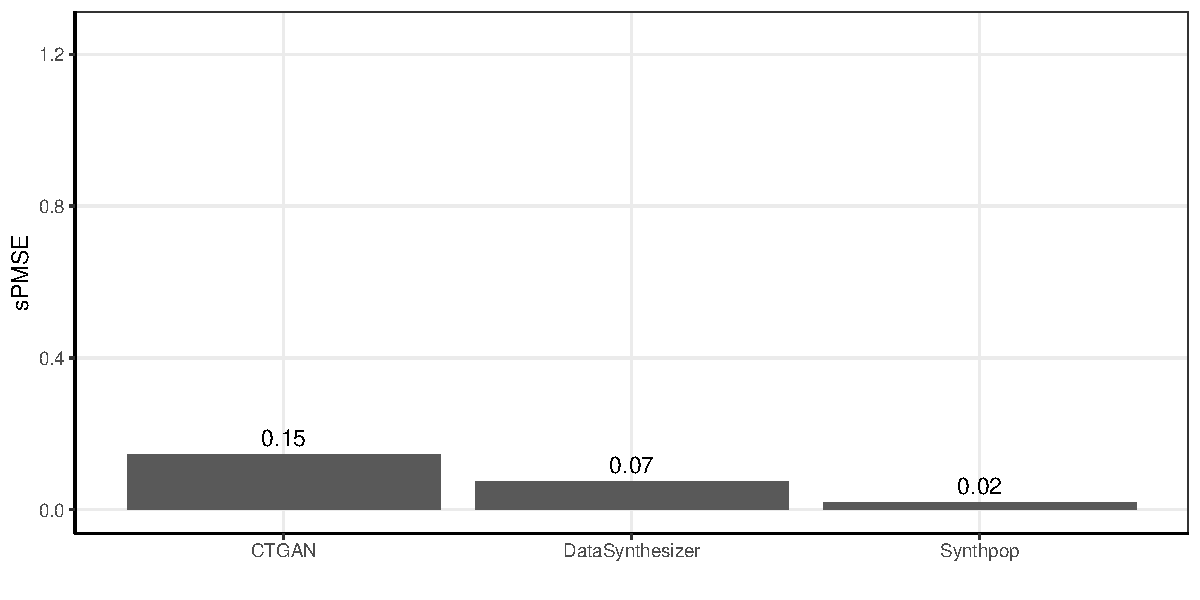
\includegraphics{../graphs/graph_fidelity_compare_dataset.pdf}}
        \label{subfig:graph_fidelity_compare_dataset}
    \end{subfigure}

    \begin{subfigure}{\textwidth}
        \caption{Two-way pMSE}
        \resizebox{\textwidth}{!}{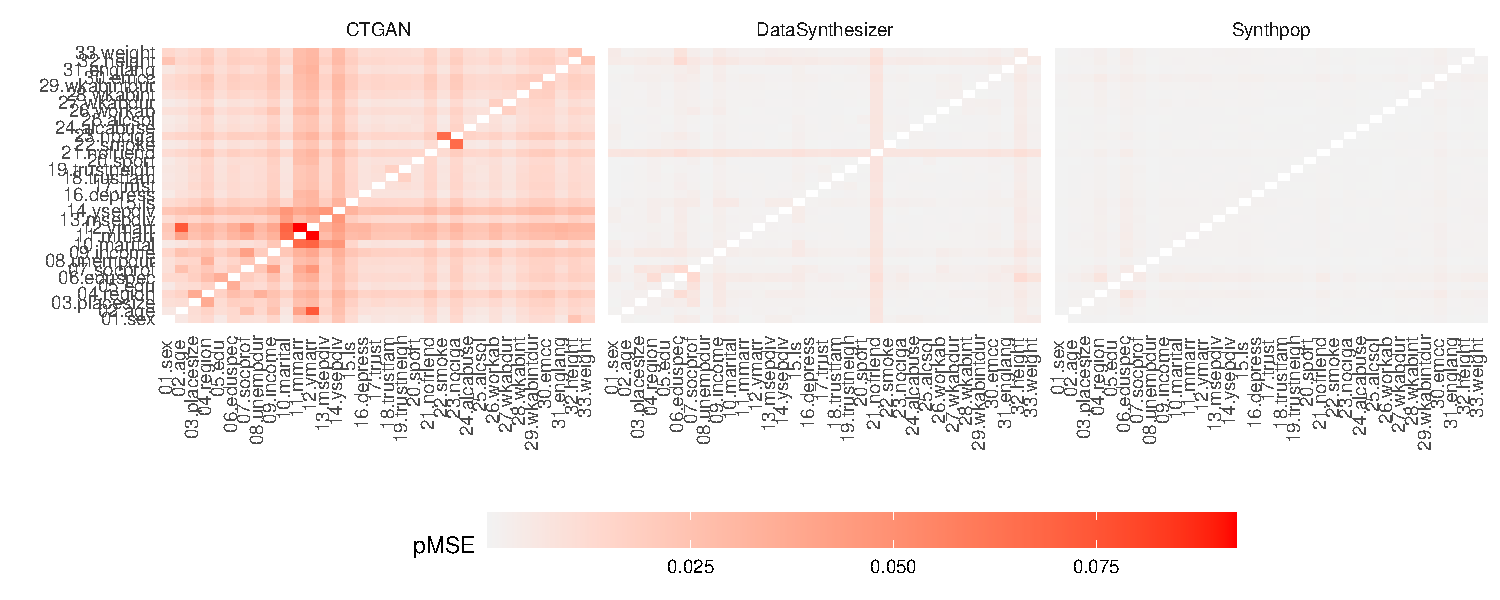
\includegraphics{../graphs/graph_fidelity_twoway_compare.pdf}}
        \label{subfig:graph_fidelity_compare_twoway}
    \end{subfigure}
\end{figure}


\begin{figure}[ht]
    \caption{Comparing one-way frequency of select variables and ROE}
    \label{fig:graph_frequency_compare}
    \centering

    \begin{subfigure}{\textwidth}
        \centering        
        \caption{Number of friends}
        \resizebox{.9\textwidth}{!}{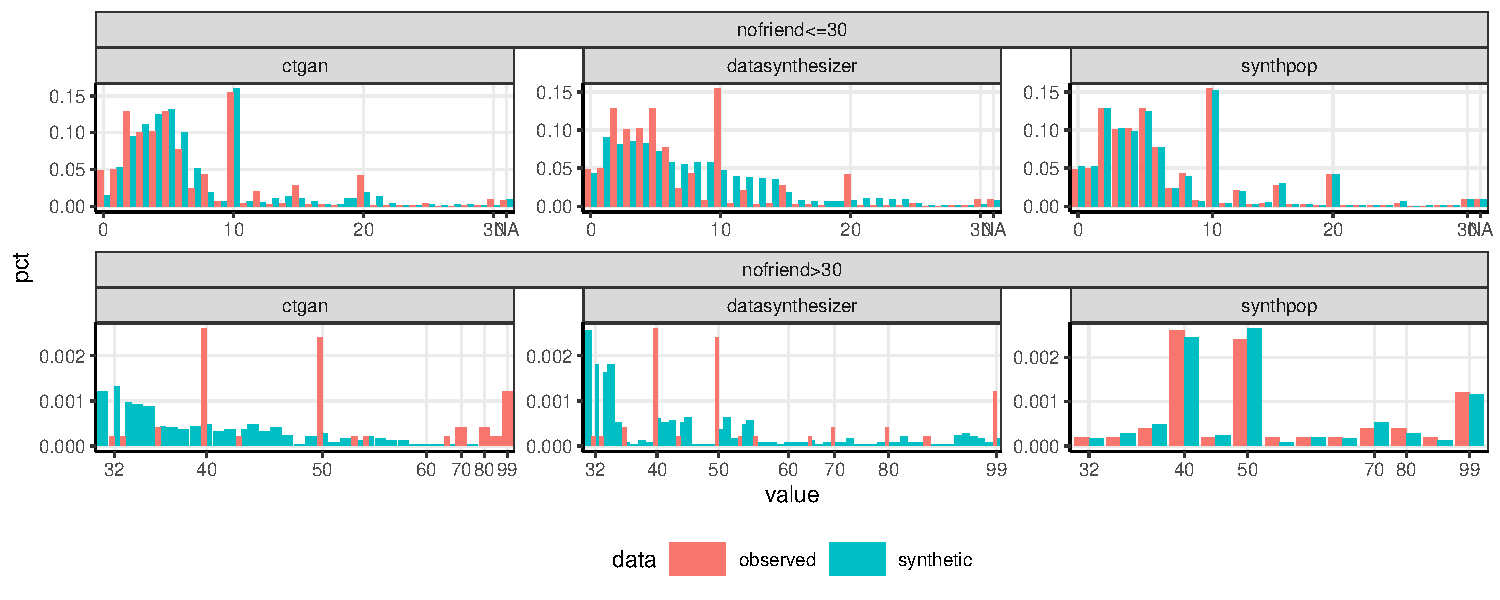
\includegraphics{../graphs/compare_nofriend_1.pdf}}
        \label{subfig:graph_frequency_compare_nofriend}
    \end{subfigure}

    \begin{subfigure}{\textwidth}
        \centering        
        \caption{BMI}
        \resizebox{.9\textwidth}{!}{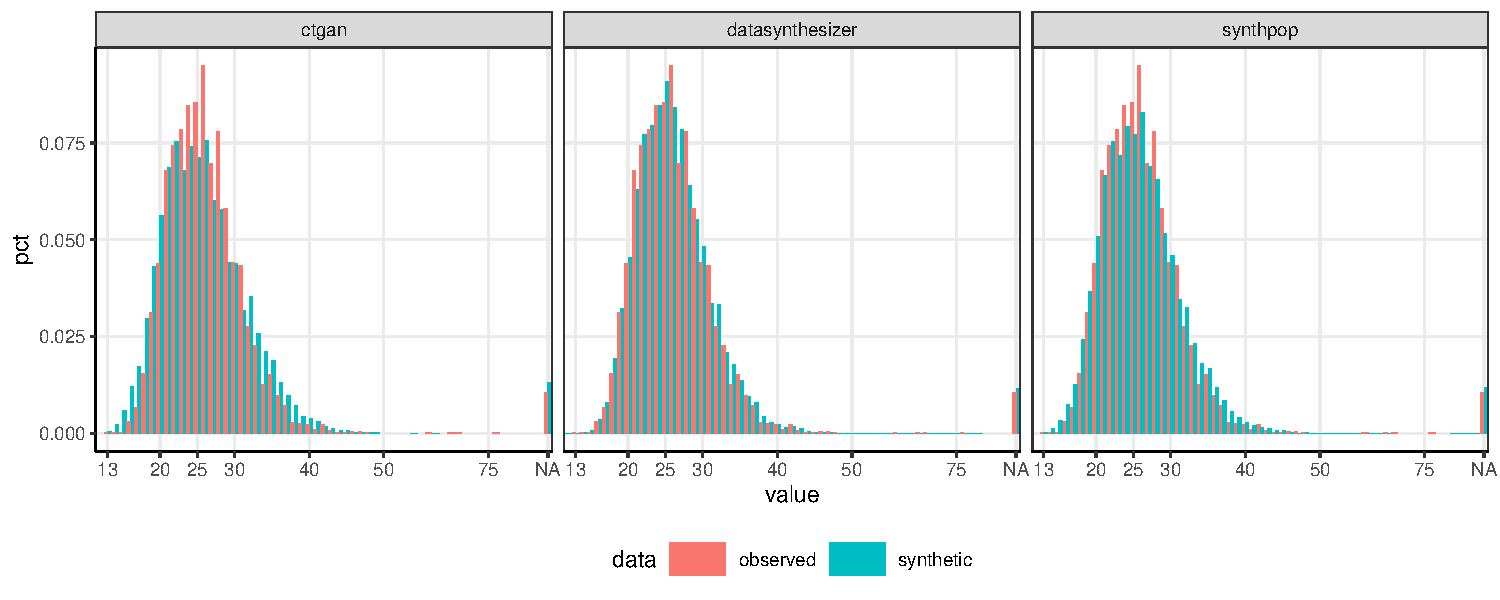
\includegraphics{../graphs/compare_bmi_1.pdf}}
        \label{subfig:graph_frequency_compare_bmi}
    \end{subfigure}

    \begin{subfigure}{\textwidth}
        \centering        
        \caption{Work abroad duration}
        \resizebox{.9\textwidth}{!}{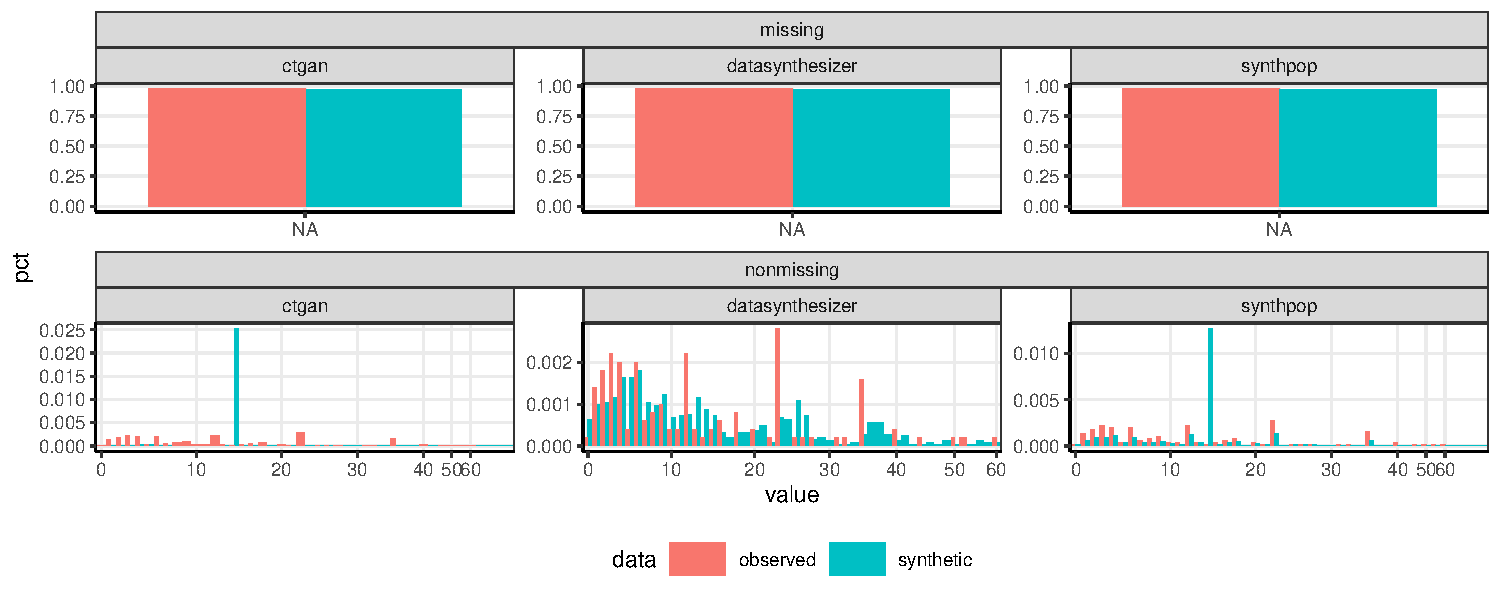
\includegraphics{../graphs/compare_wkabdur_1.pdf}}
        \label{subfig:graph_frequency_compare_wkabdur}
    \end{subfigure}

    \begin{subfigure}{\textwidth}
        \centering        
        \caption{Ratio of estimates (ROE)}
        \resizebox{.9\textwidth}{!}{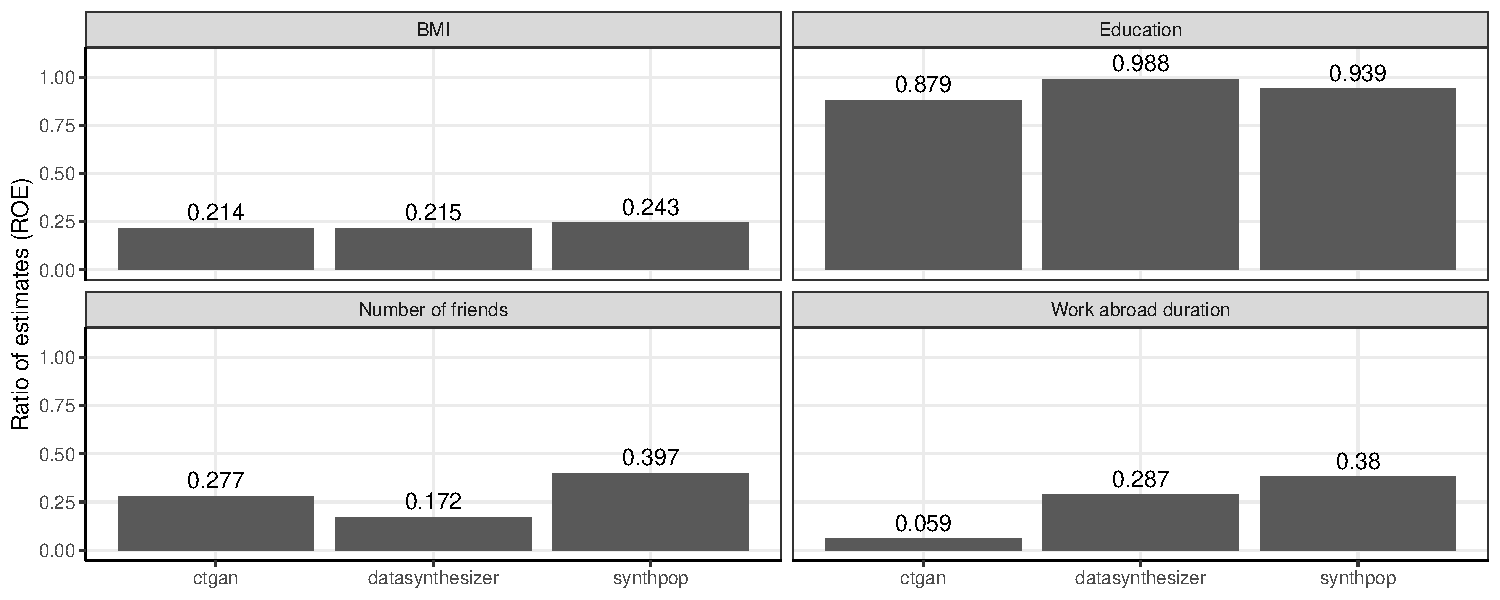
\includegraphics{../graphs/graph_compare_roe.pdf}}
        \label{subfig:graph_compare_roe}
    \end{subfigure}
\end{figure}

\begin{figure}
    \caption{Confidence interval overlap}
    \resizebox{\textwidth}{!}{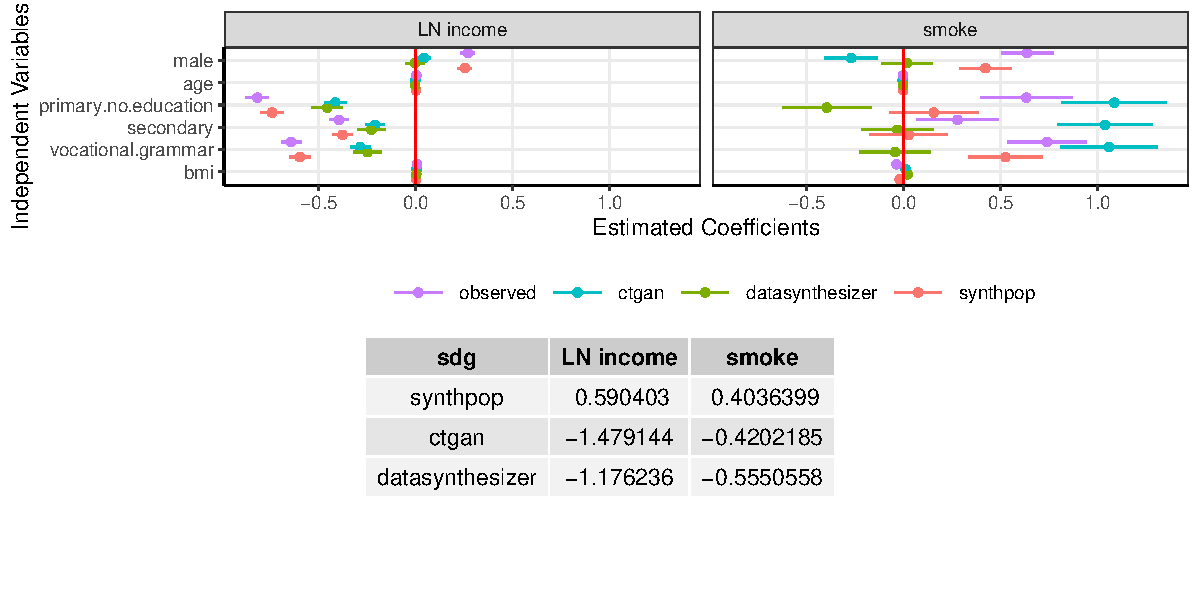
\includegraphics{../graphs/graph_utility_regression_cio_both.pdf}}
    \label{fig:utility_compare_cio}
\end{figure}


%%%%%%%%%%%%%%%%%%%%%%%%%%%%%%%%
% Bibliography
%%%%%%%%%%%%%%%%%%%%%%%%%%%%%%%%
\clearpage
\bibliographystyle{splncs04}
\bibliography{references}

%%%%%%%%%%%%%%%%%%%%%%%%%%%%%%%%
% Appendix
%%%%%%%%%%%%%%%%%%%%%%%%%%%%%%%%
\clearpage
\appendix
%%%%%%%%%%%%%%%%%%%%%%%%%%%%%%%%%%%%%%
%%%%%%%%%%%%%%%%%%%%%%%%%%%%%%%%%%%%%%
%Table
%%%%%%%%%%%%%%%%%%%%%%%%%%%%%%%%%%%%%%
%%%%%%%%%%%%%%%%%%%%%%%%%%%%%%%%%%%%%%

% \begin{table}[ht]
%     \caption{Versions of Social Diagnosis 2011 (SD2011)}
%     \centering
%     % latex table generated in R 4.3.0 by xtable 1.8-4 package
% Thu Feb  1 15:54:24 2024
\begin{tabular}{lll}
    \toprule
Data & & Description \\ \midrule
SD2011(a) && Raw data \\
SD2011(b) && + Cleaned: Missings are numeric values $<$ 0 and empty categorical cells \\
SD2011(c) && + Drop generated variables (\texttt{bmi} and \texttt{agegr}) \\
    \bottomrule
\end{tabular}

%     \label{table:sd2011_versions}
% \end{table}


%%%%%%%%%%%%%%%%%%%%%%%%%%%%%%%%%%%%%%
% Appendix
% DATASYNTHESIZER
%%%%%%%%%%%%%%%%%%%%%%%%%%%%%%%%%%%%%%
\section{Appendix: DataSynthesizer}\label{appendix:datasynethsizer}
\setcounter{figure}{0}    
\setcounter{table}{0}    
\renewcommand*\thetable{\Alph{section}.\arabic{table}}
\renewcommand*\thefigure{\Alph{section}.\arabic{figure}}
\renewcommand{\theHfigure}{\Alph{section}.\arabic{table}}
\renewcommand{\theHtable}{\Alph{section}.\arabic{figure}}

\begin{figure}[ht]
  \caption{Tuning DataSynthesizer across parents}
  \label{fig:tuning_ds}
  \centering
  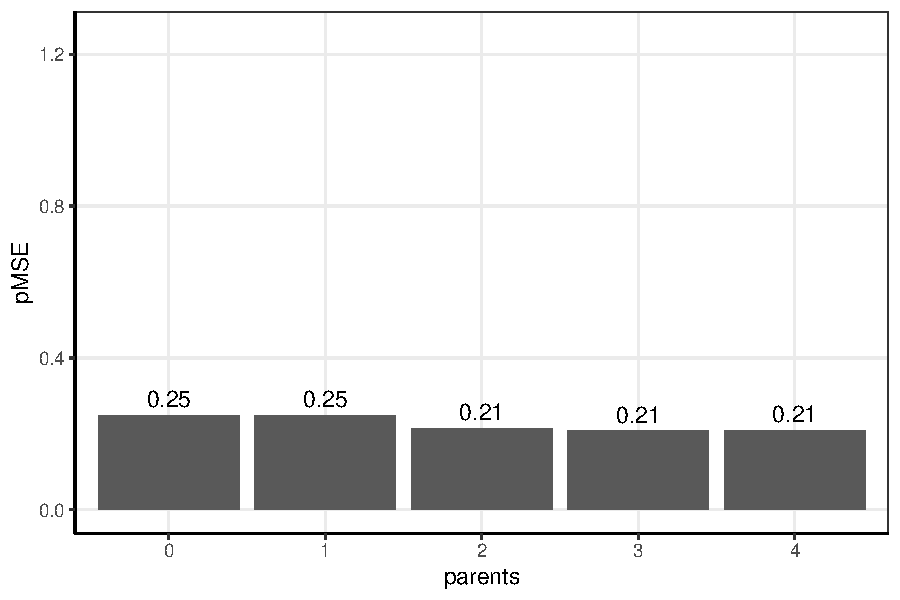
\includegraphics[width=\linewidth]{../graphs/datasynthesizer/datasynthesizer_fidelity_optimize_dataset_parents.pdf}
  \label{fig:tuning_ds_dataset}
\end{figure}

\begin{figure}[ht]
  \caption{Datasynthesizer two-way correlation  (pMSE)}
  \label{fig:ds_fidelity_two_way}
  \centering

  \begin{subfigure}{0.75\textwidth}
    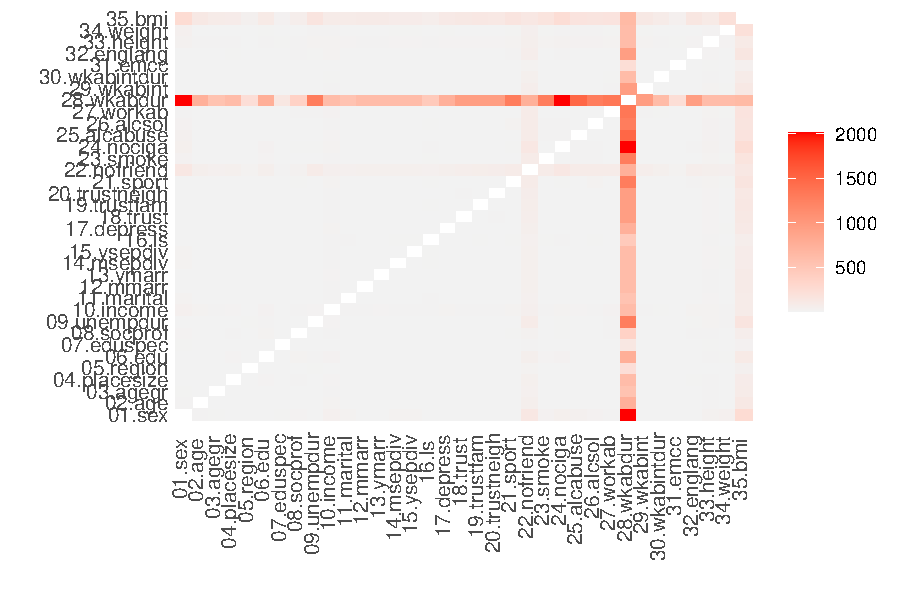
\includegraphics[width=\linewidth]{../graphs/datasynthesizer/datasynthesizer_fidelity_twoway_sd2011.pdf}
    \caption{SD2011(a)}
    \label{subfig:ds_fidelity_two_way_subfig-a}
  \end{subfigure}

  \begin{subfigure}{0.75\textwidth}
    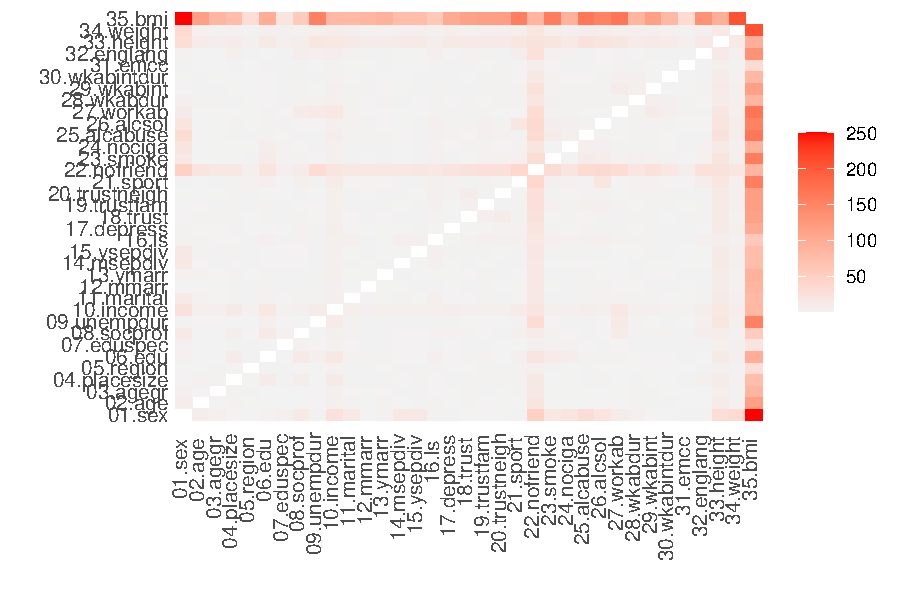
\includegraphics[width=\linewidth]{../graphs/datasynthesizer/datasynthesizer_fidelity_twoway_sd2011_clean.pdf}
    \caption{SD2011(b)}
    \label{subfig:ds_fidelity_two_way_subfig-b}
  \end{subfigure}

  \begin{subfigure}{0.75\textwidth}
    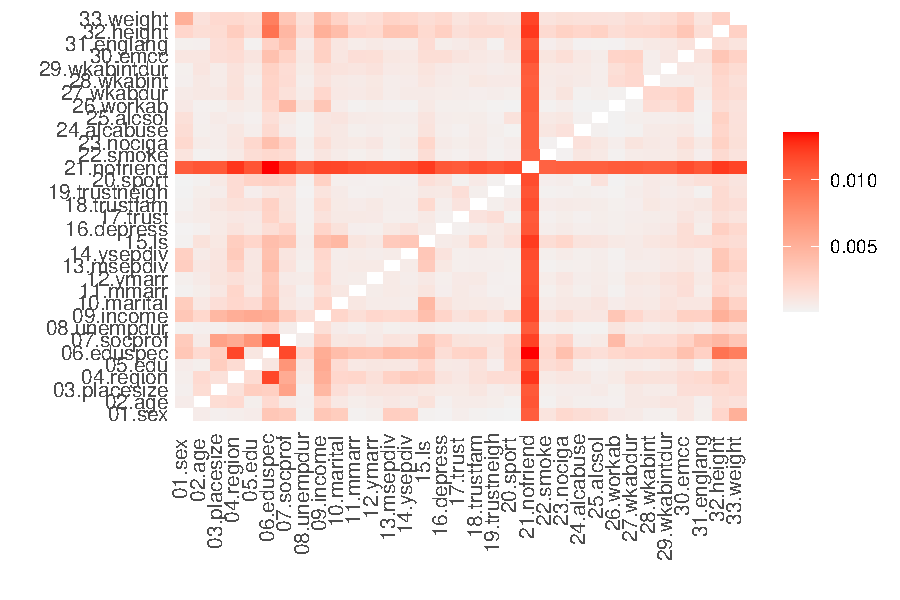
\includegraphics[width=\linewidth]{../graphs/datasynthesizer/datasynthesizer_fidelity_twoway_sd2011_clean_small.pdf}
    \caption{SD2011(c)}
    \label{subfig:ds_fidelity_two_way_subfig-c}
  \end{subfigure}
\end{figure}

\begin{figure}[ht]
  \caption{Frequency values for original and synthetic data (DataSynthesizer)}
  \label{fig:ds_variables}
  \centering

\begin{subfigure}{\textwidth}
    \caption{Variable: \texttt{wkabdur} (Work abroad duration)}
    \resizebox{\textwidth}{!}{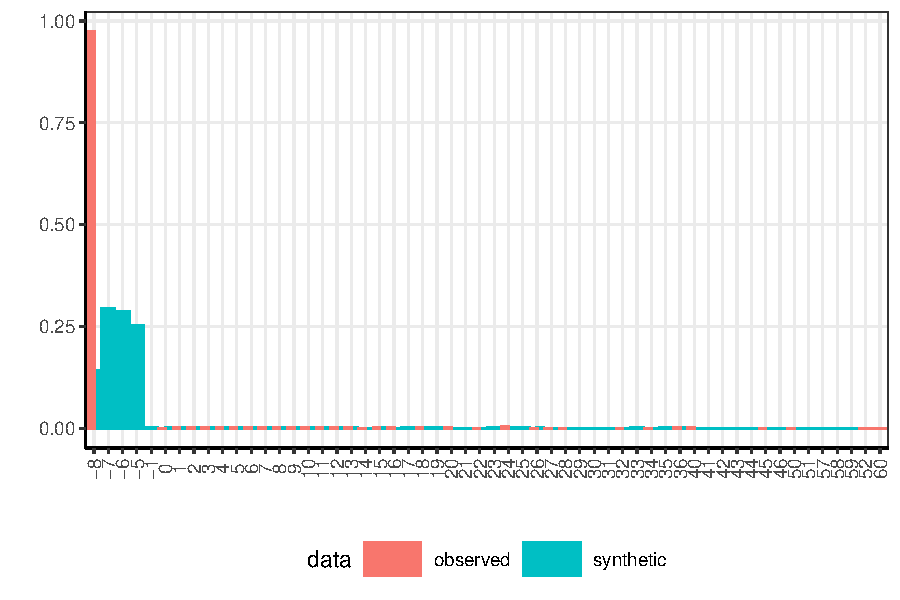
\includegraphics{../graphs/datasynthesizer/datasynthesizer_wkabdur.pdf}}
    \label{subfig:ds_variable_wkabdur}
\end{subfigure}

\begin{subfigure}{\textwidth}
    \caption{Variable: \texttt{bmi} (Body mass index)}
    \resizebox{\textwidth}{!}{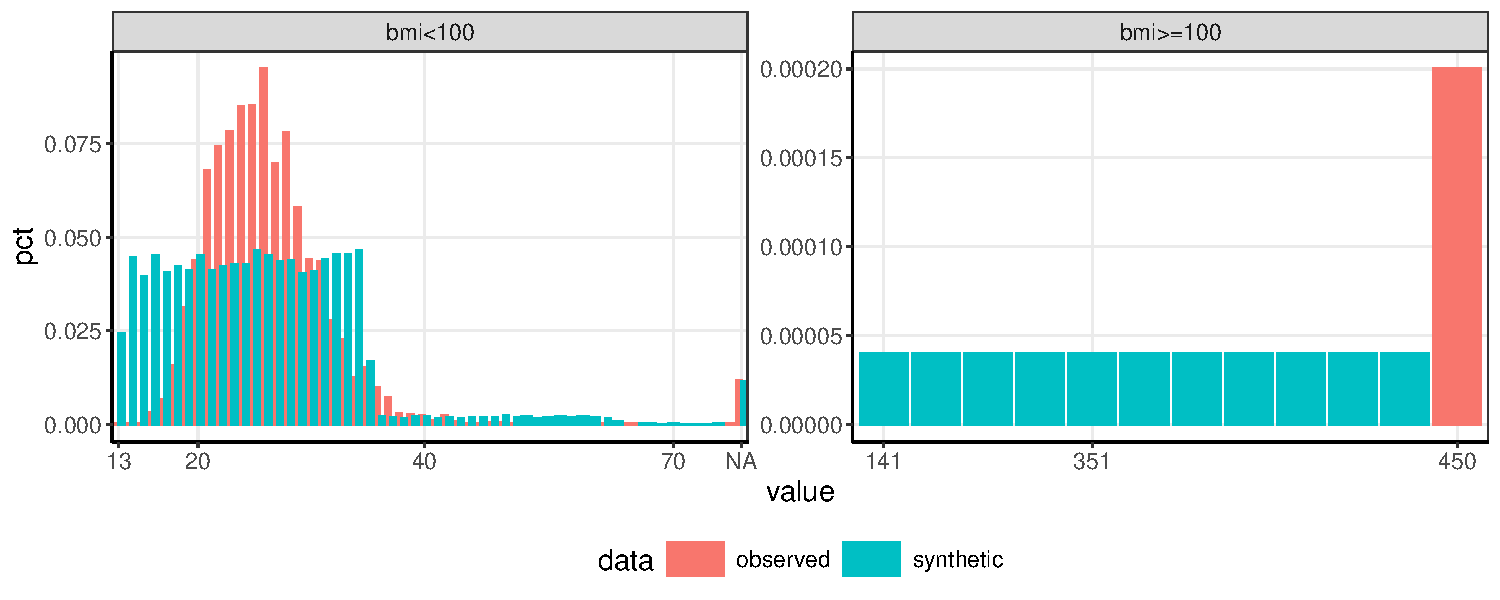
\includegraphics{../graphs/datasynthesizer/datasynthesizer_bmi.pdf}}
    \label{subfig:ds_variable_bmi}
\end{subfigure}


\begin{subfigure}{\textwidth}
    \caption{Variable: \texttt{nofriend} (Number of friends)}
    \resizebox{\textwidth}{!}{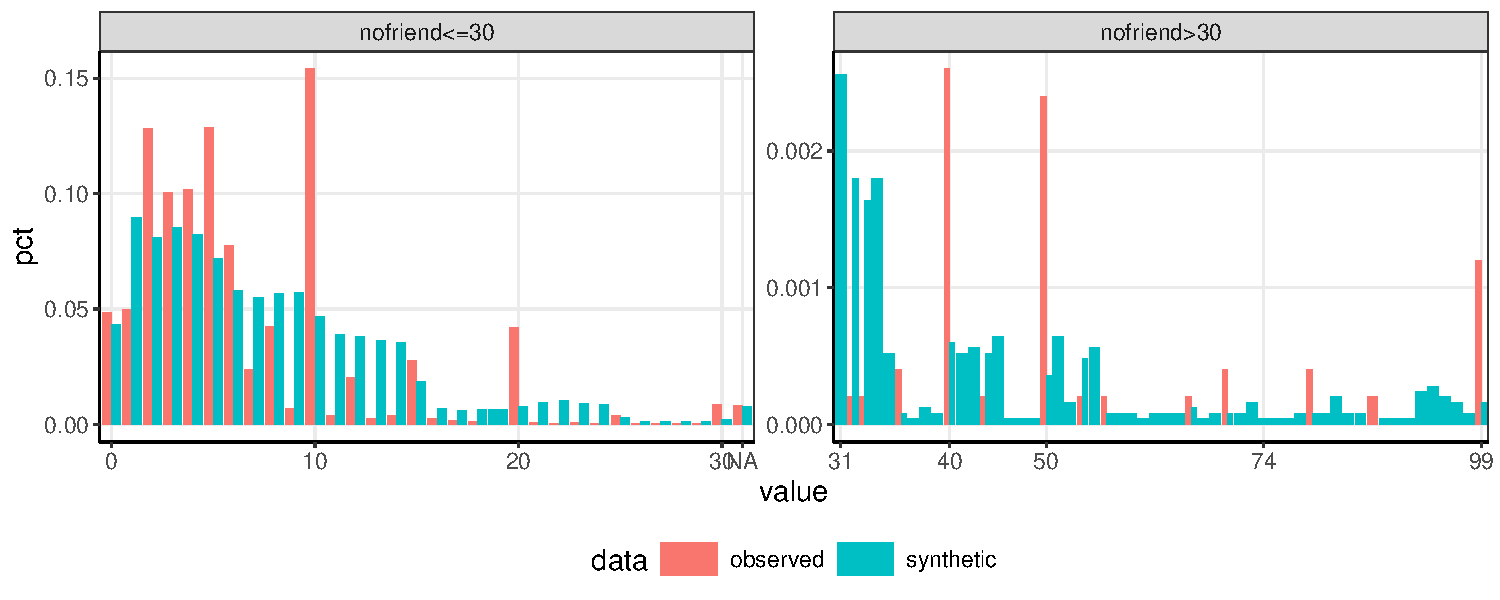
\includegraphics{../graphs/datasynthesizer/datasynthesizer_nofriend.pdf}}
    \label{subfig:ds_variable_nofriend}
\end{subfigure}
\end{figure}

\begin{figure}[ht]
  \caption{Tuning DataSynthesizer across data sets (parents = 2)}
  \label{fig:tuning_ds}
  \centering
  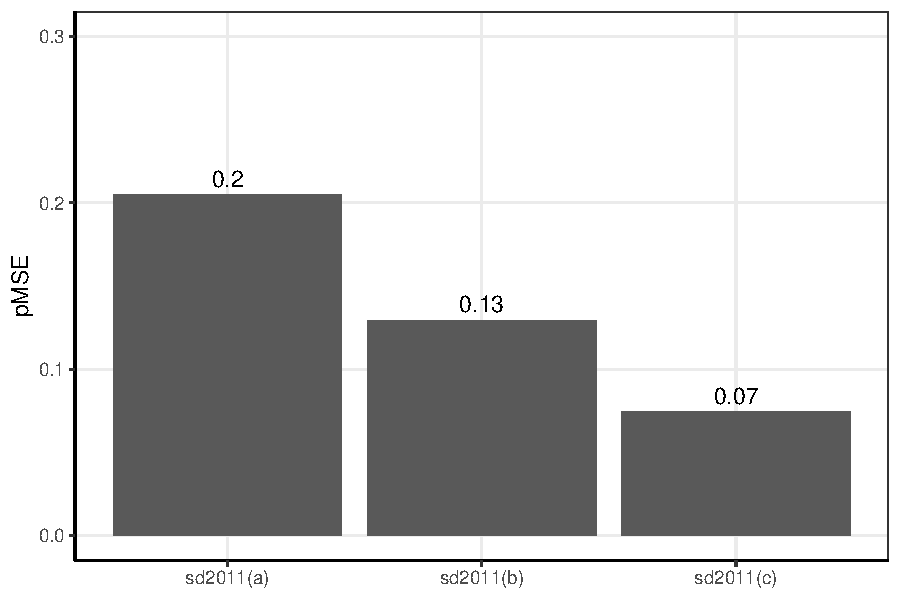
\includegraphics[width=\linewidth]{../graphs/datasynthesizer/datasynthesizer_fidelity_optimize_dataset_compare.pdf}
  \label{fig:tuning_ds_optimize_dataset_compare}
\end{figure}


%%%%%%%%%%%%%%%%%%%%%%%%%%%%%%%%%%%%%%
% Appendix
% CTGAN
%%%%%%%%%%%%%%%%%%%%%%%%%%%%%%%%%%%%%%
\clearpage
\section{Appendix: CTGAN}\label{appendix:CTGAN}
\setcounter{figure}{0}    
\setcounter{table}{0}    
\renewcommand*\thetable{\Alph{section}.\arabic{table}}
\renewcommand*\thefigure{\Alph{section}.\arabic{figure}}
\renewcommand{\theHfigure}{\Alph{section}.\arabic{table}}
\renewcommand{\theHtable}{\Alph{section}.\arabic{figure}}

\begin{table}[!h]
    \rowcolors{1}{white}{lightgray}
    \caption{Batch size and epochs = total steps}
    \centering
    \begin{tabular}{cllll>{\cellcolor{white}}p{1in}}
    % {cllllp{1in}}
    \toprule
    N & Batch size & Steps per Epoch & Epochs & Total Steps & Compare \\
    \midrule
    5.000 & 500 & 10 & 100 & 1,000 & \multirow{4}{1in}{Constant batch size, as shown in figure \ref{subfig:ctgan_fidelity_optimize_batch_size}}\\
    5.000 & 500 & 10 & 300 & 3,000 \\
    5.000 & 500 & 10 & 600 & 6,000 \\
    5.000 & 500 & 10 & 900 & 9,000 \\ \hline
    5.000 & 100 & 50 & 60 & 3,000  & \multirow{4}{1in}{Constant batch size, as shown in figure \ref{subfig:ctgan_fidelity_optimize_epochs}} \\
    5.000 & 250 & 20 & 150 & 3,000 \\
    5.000 & 500 & 10 & 300 & 3,000 \\
    5.000 & 1.000 & 5 & 600 & 3,000 \\ 
    \bottomrule
    \end{tabular}
\end{table}

\begin{figure}[ht]
  \caption{Tuning CTGAN (effect of steps)}
  \label{fig:ctgan_fidelity_optimize}
  \centering

  \begin{subfigure}{0.75\textwidth}
  \caption{Effect of batch size with constant steps (3.000)}
  \resizebox{\textwidth}{!}{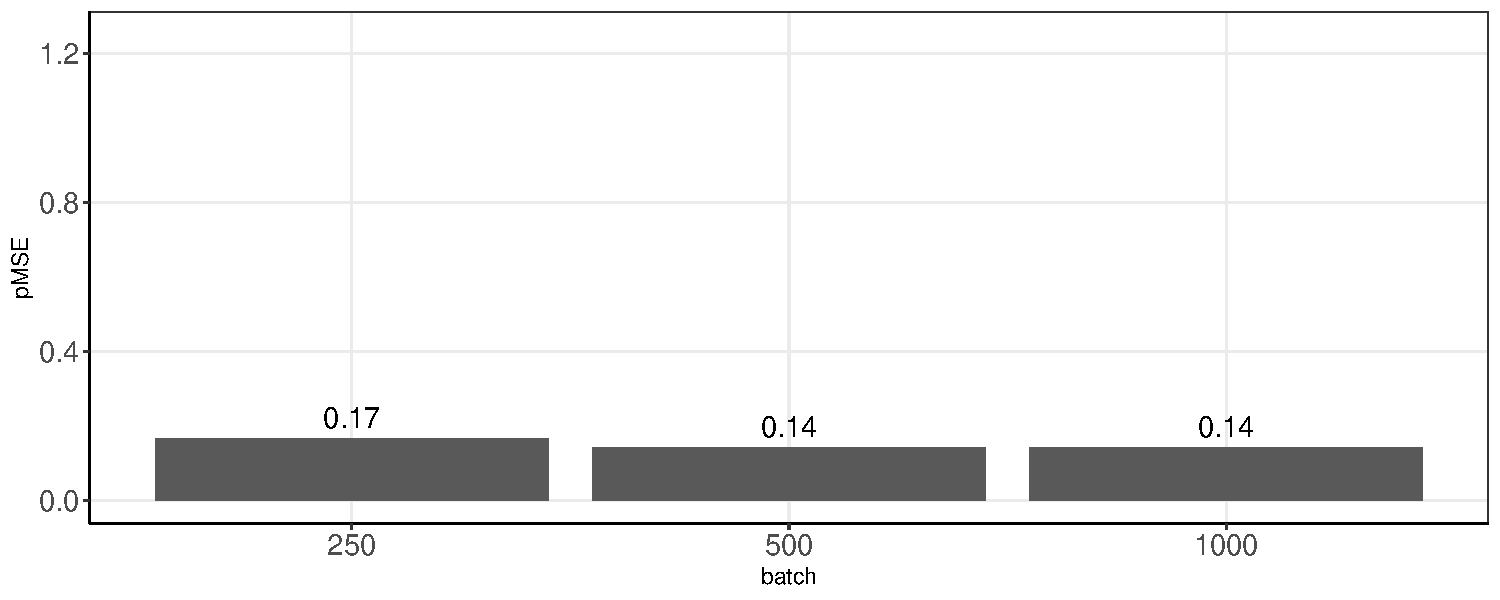
\includegraphics{../../ctgan/graphs/ctgan/ctgan_fidelity_optimize_batch_size.pdf}}
  \label{subfig:ctgan_fidelity_optimize_batch_size}
  \end{subfigure}

  \begin{subfigure}{0.75\textwidth}
  \caption{Effect of epoch number with constant batch size (500)}
  \resizebox{\textwidth}{!}{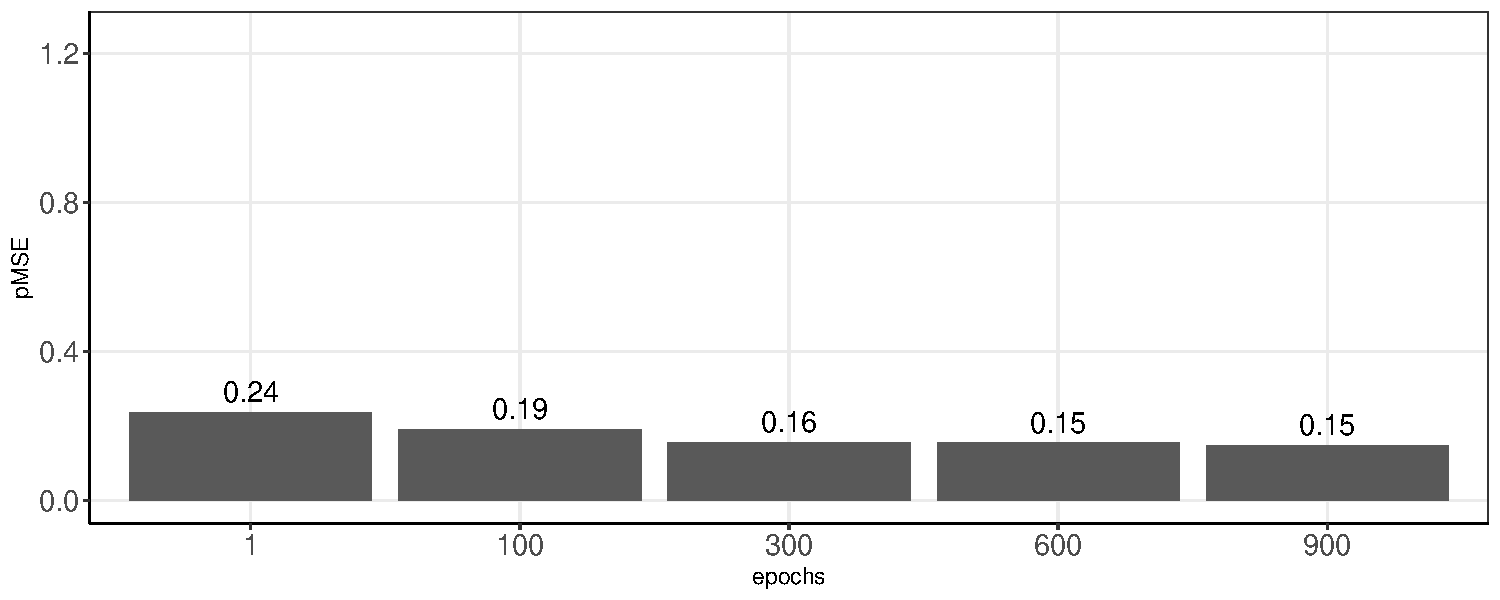
\includegraphics{../../ctgan/graphs/ctgan/ctgan_fidelity_optimize_epochs.pdf}}
  \label{subfig:ctgan_fidelity_optimize_epochs}
  \end{subfigure}

  \begin{subfigure}{0.75\textwidth}
    \caption{Effect of dimensionality}
      \resizebox{\textwidth}{!}{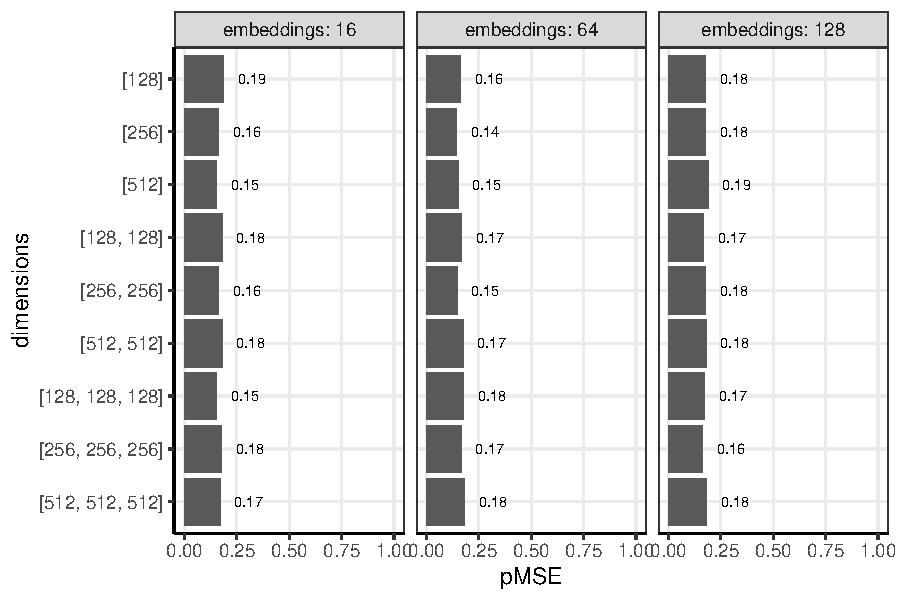
\includegraphics{../../ctgan/graphs/ctgan/ctgan_fidelity_optimize_dimensions.pdf}}
      \label{subfig:ctgan_fidelity_optimize_dimensions}
  \end{subfigure}
\end{figure}


\begin{figure}[ht]
  \caption{CTGAN two-way correlation (pMSE)}
  \label{fig:ctgan_fidelity_two_way}
  \centering

  \begin{subfigure}{0.75\textwidth}
    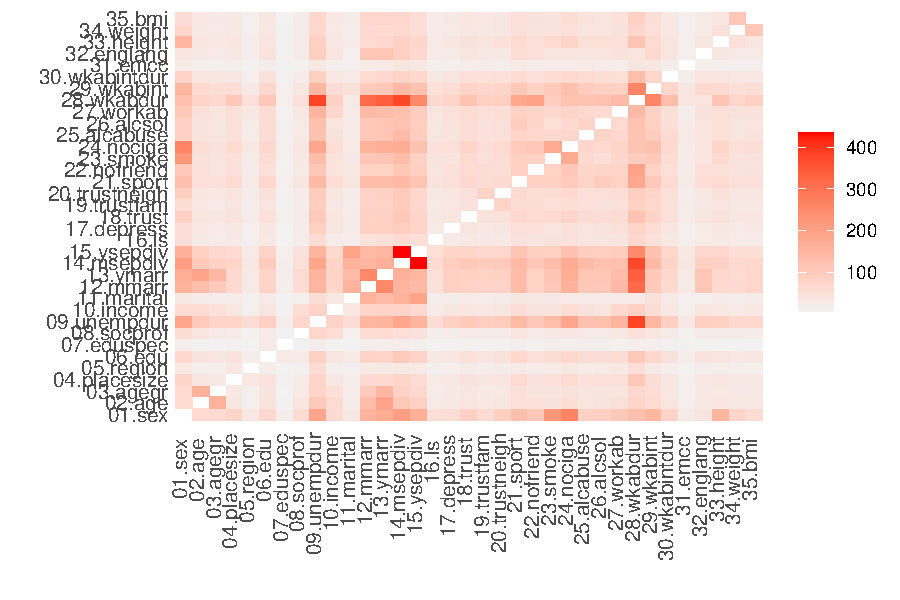
\includegraphics[width=\linewidth]{../graphs/ctgan/ctgan_fidelity_twoway_sd2011.pdf}
    \caption{SD2011(a)}
    \label{fig:ctgan_fidelity_two_way_subfig-a}
  \end{subfigure}

  \begin{subfigure}{0.75\textwidth}
    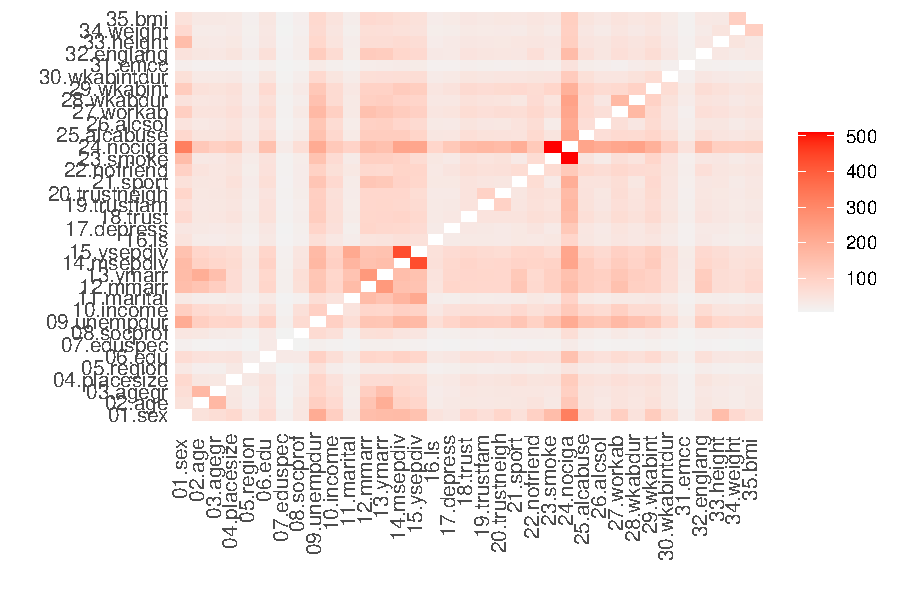
\includegraphics[width=\linewidth]{../graphs/ctgan/ctgan_fidelity_twoway_sd2011_clean.pdf}
    \caption{SD2011(b)}
    \label{fig:ctgan_fidelity_two_way_subfig-b}
  \end{subfigure}

  \begin{subfigure}{0.75\textwidth}
    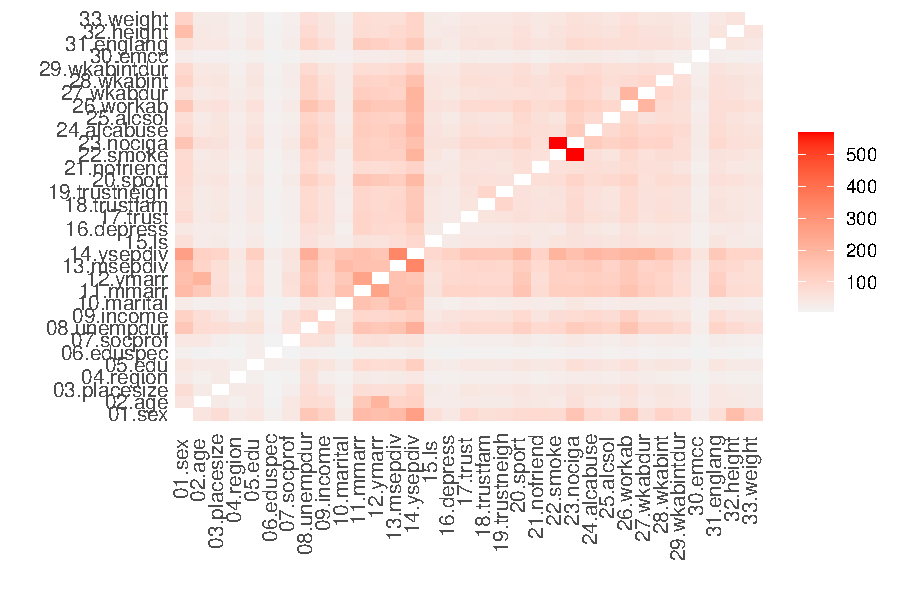
\includegraphics[width=\linewidth]{../graphs/ctgan/ctgan_fidelity_twoway_sd2011_clean_small.pdf}
    \caption{SD2011(c)}
    \label{fig:ctgan_fidelity_two_way_subfig-c}
  \end{subfigure}

\end{figure}

%%%%%%%%%%%%%%%%%%%%%%%%%%%%%%%%%%%%%%
%%%%%%%%%%%%%%%%%%%%%%%%%%%%%%%%%%%%%%
%SYNTHPOP
%%%%%%%%%%%%%%%%%%%%%%%%%%%%%%%%%%%%%%
%%%%%%%%%%%%%%%%%%%%%%%%%%%%%%%%%%%%%%
\begin{figure}[ht]
  \caption{Synthpop two-way correlation  (pMSE)}
  \label{fig:synthpop_fidelity_two_way}
  \centering

  \begin{subfigure}{0.75\textwidth}
    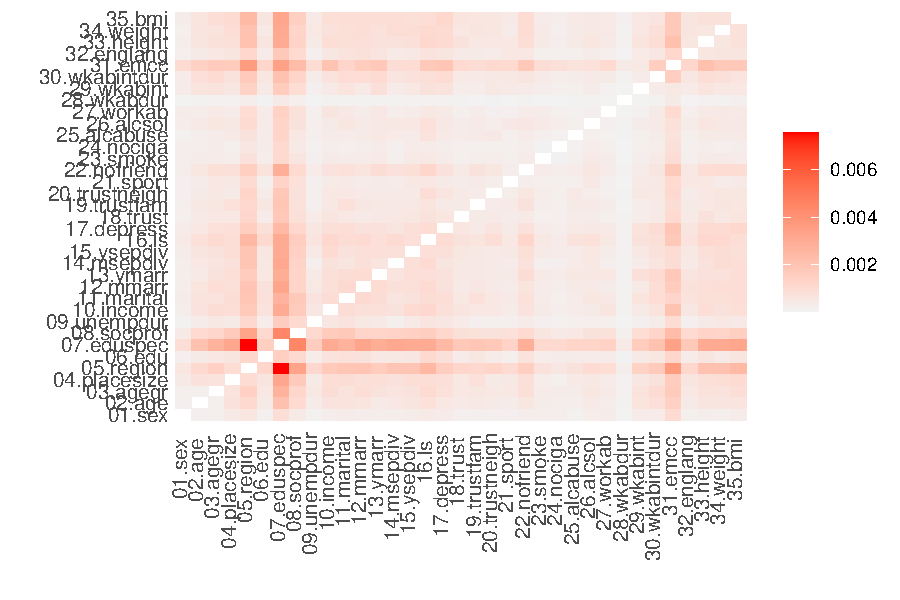
\includegraphics[width=\linewidth]{../graphs/synthpop/synthpop_fidelity_twoway_sd2011.pdf}
    \caption{SD2011(a)}
    \label{fig:synthpop_fidelity_two_way_subfig-a}
  \end{subfigure}

  \begin{subfigure}{0.75\textwidth}
    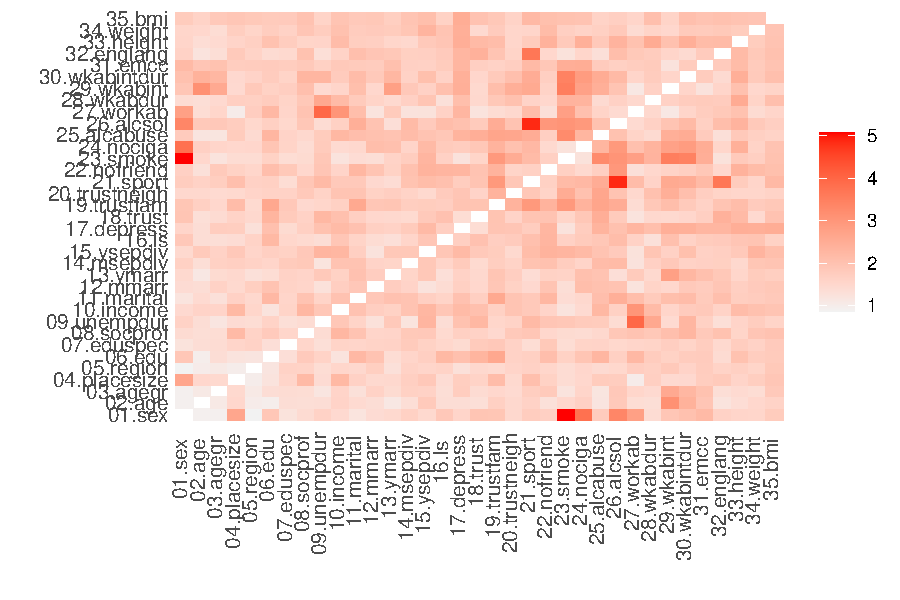
\includegraphics[width=\linewidth]{../graphs/synthpop/synthpop_fidelity_twoway_sd2011_clean.pdf}
    \caption{SD2011(b)}
    \label{fig:synthpop_fidelity_two_way_subfig-b}
  \end{subfigure}

  \begin{subfigure}{0.75\textwidth}
    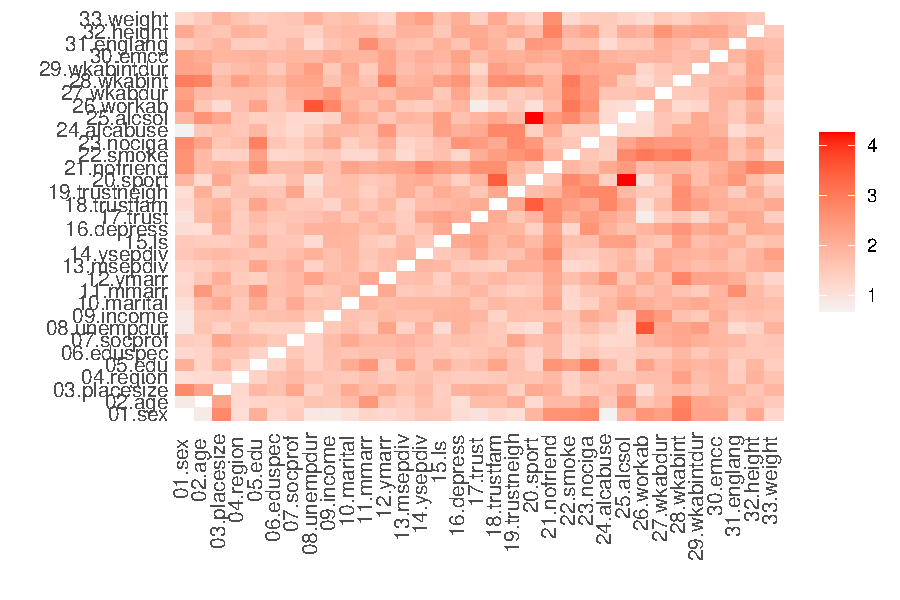
\includegraphics[width=\linewidth]{../graphs/synthpop/synthpop_fidelity_twoway_sd2011_clean_small.pdf}
    \caption{SD2011(c)}
    \label{fig:synthpop_fidelity_two_way_subfig-c}
  \end{subfigure}

\end{figure}



\end{document}
